\setchaptergraphic{}

\chapter{Differential Geometry}
\label{ch:diffgeo}

\section{Curves}

\begin{defn}
    Let $U \subseteq \R^n$ be an open set, and $f: U \to \R^m$ a function on $U$. If $f$ has continuous (mixed) partial derivatives of all orders, we say $f$ is \emph{smooth}.
\end{defn}

\begin{defn}
    Let $U \subseteq \R^n$ and $V \subseteq \R^m$ be open sets. If $f: U \to V$ is smooth, bijective, and has a smooth inverse, then we say $f$ is a \emph{diffeomorphism}.
\end{defn}

\begin{prop}
    Given a diffeomorphism $f: U \to V$ and a point $x \in U$, the differential $df_x$ at $x$ is a linear isomorphism between $\R^n$ and $\R^m$.
\end{prop}

\begin{proof}
    We know that
    \begin{align*}
        \frac{\partial}{\partial x_i}\left(f \circ f^{-1}\right) = \left(\frac{\partial}{\partial x_i}f\right) \circ f^{-1} + f \circ \left(\frac{\partial}{\partial x_i}f^{-1}\right).
    \end{align*}
    Of course, $f \circ f^{-1}$ is the identity function, so this derivative is zero. Therefore,
    \begin{align*}
        \left(\frac{\partial}{\partial x_i}f\right) \circ f^{-1} = -f \circ \left(\frac{\partial}{\partial x_i}f^{-1}\right).
    \end{align*}
    Similarly, expanding $f^{-1} \circ f$ we get
    \begin{align*}
        \left(\frac{\partial}{\partial x_i}f^{-1}\right) \circ f = -f^{-1} \circ \left(\frac{\partial}{\partial x_i}f\right).
    \end{align*}
\end{proof}

\begin{thm}{Inverse Function Theorem}\label{thm:inverse-function}\proofbreak
    Let $S \subseteq \R^n$ be an open set, and $f: S \to \R^n$. If $df_x$ is a linear isomorphism at $x \in S$, then there exists a neighborhood $U$ of $x$ and $V$ of $f(x)$ such that $f(U) \subseteq V$ and $f: U \to V$ is a diffeomorphism.
\end{thm}

\begin{defn}
    A \emph{parameterized curve} in $\R^n$ is a map $\alpha: I \to \R^n$, where $I$ is a convex subset (interval) of $\R$.

    We say the curve is \emph{smooth} when $\alpha$ is smooth on the interior of $I$.
\end{defn}

\begin{defn}
    The \emph{trace} of a curve $\alpha: I \to \R^n$ is the image $\alpha(I)$.
\end{defn}

\begin{defn}
    A \emph{regular} curve is a smooth parameterized curve whose differential is non-zero everywhere. If $\alpha'(t) = \vec{0}$, then we say $t$ is a \emph{singular point} of the curve.
\end{defn}

\begin{figure}[ht!]
    \centering
    \begin{tikzpicture}[scale=1.0]
        \begin{axis}[
            axis x line=middle,
            axis y line=middle,
            ymin=-5,ymax=5,ylabel=$y$,
            xmin=-5,xmax=5,xlabel=$x$
            ]
        \addplot[domain=-6:6, black, ultra thick, samples=100, variable=\t] ({t^3}, {t^2});
    \end{axis}
    \end{tikzpicture}
\caption{Smooth curve with a singular point at $t = 0$, given by $\alpha(t) = (t^3, t^2)$}
\label{fig:non-regular-curve}
\end{figure}

\begin{defn}
    A curve $\alpha: I \to \R^n$ is piecewise smooth if it is continuous, and there exist a finite number of points $t_1 < t_2 < \cdots < t_k$ such that $\alpha$ is smooth when restricted to each of $(t_1, t_2), (t_2, t_3), \ldots, (t_{k-1}, t_k)$.
\end{defn}

\begin{defn}
    The \emph{arclength} of a piecewise smooth curve $\alpha: I \to \R^n$ is
    \begin{align*}
        \ell(\alpha) = \int_{I}\norm{\alpha'(s)}ds.
    \end{align*}
\end{defn}

\begin{defn}
    Let $\alpha: I \to \R^n$ and $\beta: J \to \R^n$ both be smoothed parameterized curves. We say $\beta$ is a re-parameterization of $\alpha$ if there exists a diffeomorphism $\varphi: J \to I$ such that $\beta = \alpha \circ \varphi$. Note that we then have $\alpha = \beta \circ \varphi^{-1}$, so $\alpha$ is equivalently a re-parameterization of $\beta$.
\end{defn}

\begin{prop}
    Suppose that $\alpha: (a, b) \to \R^n$ is a regular curve. Then $\psi: (a, b) \to (0, \ell(\alpha))$ given by
    \begin{align*}
        \psi(t) \mapsto \int_{a}^{t}\norm{\alpha'(s)}ds
    \end{align*}
    is a diffeomorphism.
\end{prop}

\begin{proof}
    Since $\alpha$ is regular, $\psi$ is strictly increasing and smooth, and so has a smooth inverse.
\end{proof}

\begin{defn}
    Given a regular curve $\alpha: I \to \R^n$, the map $\beta: (0, \ell(\alpha)) \to \R^n$ given by $\beta = \alpha \circ \psi^{-1}$ (where $\psi$ is as defined above) is the \emph{arclength} parameterization of $\alpha$.
\end{defn}

\begin{defn}
    A curve $\alpha: I \to \R^n$ has \emph{unit speed} if $\norm{\alpha'(t)} = 1$ for all $t \in I$.
\end{defn}

\begin{prop}
    The arclength parameterization always has unit speed.
\end{prop}

\begin{proof}
    Let $\alpha: I \to \R^n$ be a regular curve, and let $\beta: (0, \ell(\alpha)) \to \R^n$ be its arclength parameterization, where $\beta = \alpha \circ \psi^{_1}$. Then
    \begin{align*}
        \beta'(s) &= \frac{\alpha'(s)}{\psi'(s)} \\
        \norm{\beta'(s)} &= \frac{\norm{\alpha'(s)}}{\abs{\psi'(s)}} = \frac{\norm{\alpha'(s)}}{\norm{\alpha'(s)}} = 1.
    \end{align*}
\end{proof}

\begin{defn}
    The \emph{curvature} of a unit speed curve $\alpha: I \to \R^3$ is given by $\kappa(t) = \norm{\alpha''(s)}$, and the \emph{radius of curvature} is $R(s) = 1/\kappa(s)$.
\end{defn}

\begin{prop}
    The curvature of a regular curve $\alpha: I \to \R^3$ is given by
    \begin{align*}
        \kappa(s) = \frac{\norm{\alpha_{tt} \times \alpha_{t}}}{\norm{\alpha_{t}}^3}.
    \end{align*}
\end{prop}

\begin{lemma}
    Suppose $\alpha: I \to \R^n$ is a unit speed curve. Then $\alpha'': I \to \R^n$ is everywhere orthogonal to $\alpha': I \to \R^n$.
\end{lemma}

\begin{proof}
    Notice that since $\norm{\alpha'(t)} = 1$, we can differentiate to obtain
    \begin{align*}
        0 &= \alpha'(s) \cdot \alpha''(s) + \alpha''(s) \cdot \alpha'(s) = 2\alpha'(s) \cdot \alpha''(s).
    \end{align*}
\end{proof}

\begin{defn}
    If $\alpha: I \to \R^3$ is a unit speed curve with non-zero curvature at a point $s$, define $n(s)$ to be the unit vector in the direction of $\alpha''(s)$.
\end{defn}

\begin{rmk}
    Note that the tangent vector $t(s)$ has derivative $t'(s) = \alpha''(s) = \kappa(s)n(s)$.
\end{rmk}

\begin{defn}
    Let $\alpha: I \to \R^3$ be a unit speed curve whose curvature is nowhere zero. Given the tangent and normal vectors $t(s)$, $n(s)$, the plane containing the point $\alpha(s)$ and spanned by $t(s)$ and $n(s)$ is the \emph{osculating plane} at $s$.

    We then define the \emph{binormal} vector $b(s) = t(s) \times n(s)$. Note that all three of $t(s), n(s), b(s)$ are non-zero everywhere, and in fact form an orthonormal basis for $\R^3$.
\end{defn}

\begin{lemma}\label{lemma:binormal-derivative}
    Let $\alpha: I \to \R^3$ be a unit speed curve whose curvature is nowhere zero. Then $b'(s)$ is parallel to $n(s)$.
\end{lemma}

\begin{proof}
    Since $b(s) = t(s) \times n(s)$, we know
    \begin{align*}
        b'(s) = t'(s) \times n(s) + t(s) \times n'(s).
    \end{align*}
    Since $t'(s) = \kappa(s)n(s)$, it follows that $t'(s) \times n(s) = 0$, and so $b'(s)$ is normal to $t(s)$. Furthermore, $1 = b(s)^{\transpose}b(s)$, and so taking the derivative with respect to $s$ we find $b'(s)^{\transpose}b(s) = 0$. Therefore, $b'(s)$ is orthogonal to both $t(s)$ and $b(s)$, and is therefore a scalar multiple of $n(s)$.
\end{proof}

\begin{defn}
    The \emph{torsion} of a curve is $\tau: I \to \R$, such that $b'(s) = \tau(s)n(s)$.
\end{defn}

\begin{thm}{Frenet-Serret Formulas}\label{thm:frenet-serret}\proofbreak
    Let $\alpha: I \to \R^3$ be a unit speed curve whose curvature is nowhere zero. Then
    \begin{align*}
        t'(s) &= \kappa(s)n(s), \\
        n'(s) &= -\tau(s)b(s) - \kappa(s)t(s), \\
        b'(s) &= \tau(s)n(s). \\
    \end{align*}
\end{thm}

\begin{proof}
    The formula for $t'(s)$ comes directly from the definition of $n(s)$ and $\kappa(s)$, and the formula for $b'(s)$ come from Lemma \ref{lemma:binormal-derivative}. Finally,
    \begin{align*}
        n'(s) &= b'(s) \times t(s) + b(s) \times t'(s) \\
        &= \tau(s)n(s) \times t(s) + b(s) \times \kappa(s)n(s) \\
        &= -\tau(s)b(s) - \kappa(s)t(s).
    \end{align*}
\end{proof}

\begin{thm}{Fundamental Theorem of The Local Theory of Curves}\label{thm:local-theory-curves}\proofbreak
    Given functions $\kappa: I \to (0, \infty)$ and $\tau: I \to \R$, there exists a unit speed curve $\alpha: I \to \R^3$ such that $\kappa(s)$ and $\tau(s)$ are the curvature and torsion of $\alpha$ for all $s \in I$.

    Furthermore, given any two curves $\alpha: I \to \R^3$ and $\tilde{\alpha}: I \to \R^3$ with the same curvature and torsion, there exists a rigid motion such that $\tilde{\alpha}(s) = R\alpha(s) + t$ for a rotation matrix $R$ and translation $t \in \R^3$.
\end{thm}

\begin{proof}
    For existence, fix an arbitrary initial point and orthonormal basis $\langle t, n, b\rangle$, such as $\vec{0}$ and the standard basis. By the Cauchy-Lipschitz Theorem {\large\color{red}TODO} a unique solution exists.

    Given any two choices of initial conditions, there is clearly a rigid motion between. That is, if we fix a point $s_0 \in I$ then given two such curves $\alpha, \tilde{\alpha}$, let $t = \tilde{\alpha}(s_0) - \alpha(s_0)$, and let
    \begin{align*}
        R = \begin{bmatrix}
            | & | & | \\
            \tilde{t}(s_0) & \tilde{n}(s_0) & \tilde{b}(s_0) \\
            | & | & |
        \end{bmatrix}\begin{bmatrix}
            | & | & | \\
            t(s_0) & n(s_0) & b(s_0) \\
            | & | & |
        \end{bmatrix}^{-1}.
    \end{align*}
    Then by applying $R$ to $\tilde{\alpha}$, we obtain $t(0) = \tilde{t}(0)$, $n(0) = \tilde{n}(0)$, and $b(0) = \tilde{b}(0)$. Furthermore, by Frenet-Serret \ref{thm:frenet-serret} we have
    \begin{align*}
        \frac{1}{2}\frac{d}{ds}\left(\norm{t-\tilde{t}}^2 + \norm{n-\tilde{n}}^2 + \norm{b-\tilde{b}}^2\right) &= \langle t-\tilde{t}, t' - \tilde{t'} \rangle + \langle n-\tilde{n}, n' - \tilde{n'} \rangle + \langle b-\tilde{b}, b' - \tilde{b'} \rangle \\
        &= \langle t-\tilde{t}, \kappa n - \kappa n' \rangle + \langle n-\tilde{n}, -\tau b - \kappa t - \tau \tilde{b} - \kappa \tilde{t} \rangle + \langle b-\tilde{b},\tau n - n \tilde{n} \rangle \\
        &= \kappa \langle t-\tilde{t}, n-\tilde{n}\rangle - \kappa \langle n-\tilde{n}, t-\tilde{t}\rangle - \tau\langle n-\tilde{n},b-\tilde{b}\rangle + \tau\langle b-\tilde{b}, n-\tilde{n} \rangle \\
        &= 0.
    \end{align*}
    Since $t(0) = \tilde{t}(0)$, we find that $t(s) = \tilde{t}(s)$ for all $s \in I$. Therefore, $\alpha(s) - \alpha(0) = \tilde{\alpha}(s) - \tilde{\alpha}(0)$ is constant.
\end{proof}

\begin{defn}
    Consider a unit speed planar curve $\alpha: I \to \R^2$. The \emph{signed unit normal} $\tilde{n}$ is obtained from $t(s)$ via rotation counter-clockwise by $\pi/2$. Then the \emph{signed curvature} is $\kappa$ such that $\alpha''(s) = \kappa(s)\tilde{n}(s)$.
\end{defn}

\begin{defn}
    Let $\alpha: I \to \R^2$ be a planar unit speed curve. The \emph{signed curvature} $\kappa^{s}$ of $\alpha$ is such that $t'(s) = \kappa^{s}\tilde{n}(s)$.
\end{defn}

\begin{rmk}
    Letting $\theta(s)$ be the angle measured from the $x$-axis to $t(s)$, it follows that $t'(s) = \theta'(s)\tilde{n}(s)$.
\end{rmk}

\begin{defn}
    Given $\alpha: I \to \R^2$, where $I = (a, b)$, we can define the \emph{turning angle} $\varphi: I \to \R$ as
    \begin{align*}
        \varphi(s) = \int_{a}^{s}\kappa^{s}(\tau)d\tau.
    \end{align*}
\end{defn}

\begin{rmk}
    While $\theta(s)$ and $\varphi(s)$ are conceptually similar, they are not identical. Unlike $\theta(s)$, which may have discontinuities near the endpoints of $[0, 2\pi)$, the turning angle is continuous. Additionally, they have different initial conditions: $\varphi(0)$ is zero, while $\theta(0)$ is not generally zero.
\end{rmk}

\begin{defn}
    Let $\alpha: \R \to \R^2$ be a smooth parameterized curve. If there exists some $T > 0$ such that $\alpha(t + T) = \alpha(t$) for all $t \in \R$, we say $\alpha$ is a \emph{closed} curve. The minimum such $T$ is the \emph{period} of the curve.

    We then write $\alpha: [0, T] \to \R^2$, where $\alpha(0) = \alpha(T)$.
\end{defn}

\begin{defn}
    A \emph{Jordan curve} (or \emph{simple curve}) is a closed curve without self-intersections, i.e. if $\abs{t - s} < T$ then $\alpha(t) \neq \alpha(s)$.
\end{defn}

\begin{thm}{Smooth Schoenflies Theorem}\proofbreak
    Let $\alpha: [0, T] \to \R^2$ be a Jordan curve. Then there exists a diffeomorphism $f: \R^2 \to \R^2$ such that $f(S^1)$ coincides with the image of $\alpha$.
\end{thm}

\begin{rmk}
    Therefore, Jordan curves has an interior and exterior.
\end{rmk}

\begin{defn}
    Let $\alpha: [0, T] \to \R^2$ be a smooth closed curve. The \emph{turning number} of $\alpha$ is
    \begin{align*}
        I = \frac{1}{2\pi}\int_{0}^{T}\kappa^{s}ds.
    \end{align*}
\end{defn}

\begin{thm}
    Closed (but possible self-intersecting) curves always have integer turning number $I$.
\end{thm}

\begin{thm}
    Jordan curves always have turning number $I = \pm 1$.
\end{thm}

\begin{defn}
    A \emph{vertex} of a unit speed plane curve $\alpha: I \to \R^2$ is a stationary point of $\kappa^{s}$.
\end{defn}

\begin{thm}{Four Vertex Theorem}\label{thm:four-vertex-theorem}\proofbreak
    Every Jordan curve has \emph{at least} four vertices.
\end{thm}

\begin{defn}
    A Jordan curve is \emph{positively oriented} if the interior of the curve is on the left as the parameter increases.
\end{defn}

\begin{figure}[ht!]
    \centering
    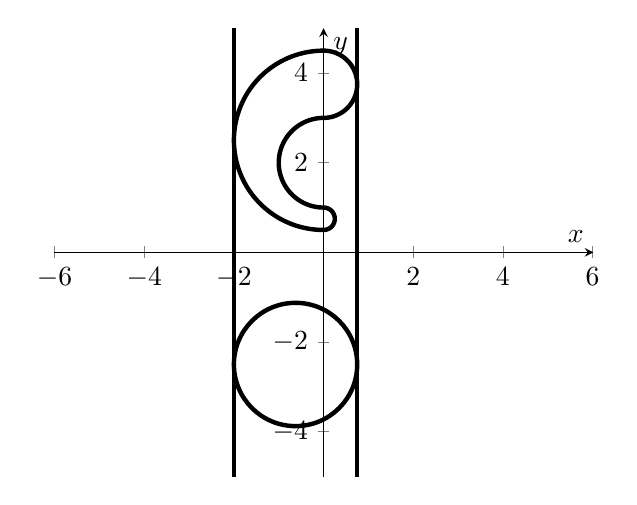
\begin{tikzpicture}[scale=1.0]
        \begin{axis}[
            axis x line=middle,
            axis y line=middle,
            axis equal,
            ymin=-5,ymax=5,ylabel=$y$,
            xmin=-5,xmax=5,xlabel=$x$
            ]
        \draw[ultra thick] (-0.625, -2.5) circle (1.375);
        \draw[ultra thick] (-2, -5) -- (-2, 5);
        \draw[ultra thick] (0.75, -5) -- (0.75, 5);

        \addplot[domain=0.25:0.75, black, ultra thick, samples=100, variable=\t] ({cos(deg(2*pi*t))}, {sin(deg(2*pi*t))+2});
        \addplot[domain=0.25:0.75, black, ultra thick, samples=100, variable=\t] ({2*cos(deg(2*pi*t))}, {2*sin(deg(2*pi*t))+2.5});
        \addplot[domain=-0.25:0.25, black, ultra thick, samples=100, variable=\t] ({0.75*cos(deg(2*pi*t))}, {0.75*sin(deg(2*pi*t))+3.75});
        \addplot[domain=-0.25:0.25, black, ultra thick, samples=100, variable=\t] ({0.25*cos(deg(2*pi*t))}, {0.25*sin(deg(2*pi*t))+0.75});
    \end{axis}
    \end{tikzpicture}
\caption{Isoperimetric inequality construction}
\label{fig:isoperimetric-construction}
\end{figure}

\begin{thm}{Isoperimetric inequality}\label{thm:isoperimetric-inequality}\proofbreak
    Among all Jordan curves $\alpha: [0, T] \to \R^2$ with the same length $T$, the circle is the unique curve attaining the maximum enclosed area.

    In particular, let $C$ be the trace of a Jordan curve with length $L$ and enclosed area $A$. Then $4\pi A \leq L^2$, with equality if and only if $C$ is a circle.
\end{thm}

\begin{proof}
    Let $v$ be an arbitary unit vector. Let $L_1$ and $L_2$ be two parallel lines, both perpendicular to $v$, and given by
    \begin{align*}
        L_1: x &= \min_{(x, y) \in C}\langle (x, y), v\rangle, \\
        L_2: x &= \max_{(x, y) \in C}\langle (x, y), v\rangle.
    \end{align*}
    Note that these maximums/minimums exist since $C$ is the continuous image of a compact set, and so is compact.

    Let $S^1$ be a circle that is tangent to both lines, and does not intersect $C$. Let $r$ be the radius of the circle, and define a coordinate system centered at $S^1$ with $y$-axis parallel to $L_1, L_2$. In this coordinate system, let $\alpha(s) = (x(s), y(s))$ be an arc-length (unit-speed) parameterization of $C$. Next, define $\tilde{y}(s) = \sqrt{r^2 - x(s)^2}$. We then define a parameterization of the circle $\tilde{\alpha}(s) = (x(s), \tilde{y}(s))$.

    Let $\tilde{A} = \pi r^2$ be the area of the circle. Using Green's Theorem, we have
    \begin{align*}
        A &= \int_{0}^{L}x(s)y'(s)ds, \\
        \tilde{A} &= -\int_{0}^{L}x'(s)\tilde{y}(s)ds.
    \end{align*}
    Therefore,
    \begin{align*}
        A + \pi r^2 &= \int_{0}^{L}xy' - x'\tilde{y}.
    \end{align*}
    By the Cauchy-Schwarz inequality,
    \begin{equation*}\tag{$\star$}\label{isoperimetric:dot-ineq}
        \abs{xy' - x'\tilde{y}} \leq \norm{\tilde{\alpha}}\norm{(y', -x')},
    \end{equation*}
    but $\norm{(y', -x')} = \norm{\alpha'} = 1$, and so
    \begin{align*}
        A + \pi r^2 \leq \int_{0}^{L}\norm{\tilde{\alpha}(t)}dt = \int_{0}^{L}rdt = rL.
    \end{align*}
    Recall that for positive $a, b$ we always have $\sqrt{ab} \leq (a + b)/2$ with equality if and only if $a = b$. Therefore,
    \begin{equation*}\tag{$\dagger$}\label{isoperimetric:area-ineq}
        \sqrt{A\pi r^2} \leq (A + \pi r^2)/2 \leq rL/2,
    \end{equation*}
    and so $A \leq L^2/(4\pi)$.

    Clearly, equality holds if $C$ is indeed a circle. It only remains to show that if equality holds, then $C$ must be a circle. For equality to hold we must have $A = \pi r^2$ in (\ref{isoperimetric:area-ineq}). Therefore, $A = L^2/(4\pi)$ gives us $L^2 = 4\pi(\pi r^2)$, and so $L = 2\pi r$. Since we could have oriented our original parallel gives $L_1, L_2$ arbitrarily by varying $v$, it must be that $C$ has constant width in all directions.

    However, just because $C$ has constant width does not mean it is a circle! For example, consider the Reuleaux triangle. However, for the equality to hold it must additionally be true that equality is attained in (\ref{isoperimetric:dot-ineq}), and so by the Cauchy-Schwarz inequality \ref{cauchy-schwarz-triangle} it follows that for all $s \in [0, L]$, there must be some $\lambda \in \R$ such that
    \begin{align*}
        \begin{pmatrix}
            x(s) \\ \tilde{y}(s)
        \end{pmatrix} &= \lambda\begin{pmatrix}
            y'(s) \\ x'(s)
        \end{pmatrix}.
    \end{align*}
    Then,
    \begin{align*}
        \lambda(s)^2 = \frac{x(s)^2 + \tilde{y}(s)^2}{x'(s)^2 + y'(s)^2} = \frac{r^2}{1}.
    \end{align*}
    In particular, $x(s) = \pm r y'(s)$. However, the parameterization of $C$ and $r$ are both independent of rotation (since $C$ is constant width), so by rotating $v$ by $pi/2$ we also have $y(s) = \pm r x'(s)$. Therefore, the curve $C$ satisfies $x^2 + y^2 = r^2y'(s)^2 + r^2x'(s)^2 = r^2$, and so is in fact a circle.
\end{proof}

\section{Surfaces}

\begin{figure}[h!]
    \centering
    \begin{minipage}[b]{0.3\linewidth}
        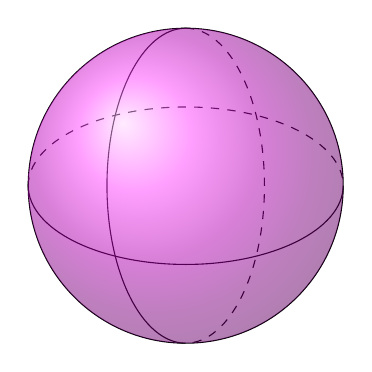
\begin{tikzpicture}
            \draw (-2,0) arc (180:360:2cm and 1cm);
            \draw[dashed] (-2,0) arc (180:0:2cm and 1cm);
            \draw (0,2) arc (90:270:1cm and 2cm);
            \draw[dashed] (0,2) arc (90:-90:1cm and 2cm);
            \draw (0,0) circle (2cm);
            \shade[ball color=Fuchsia,opacity=0.5] (0,0) circle (2cm);
        \end{tikzpicture}
    \end{minipage}
    \begin{minipage}[b]{0.3\linewidth}
        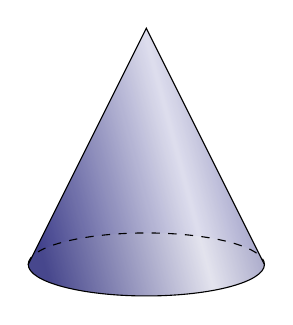
\begin{tikzpicture}
            \fill[color=blue, opacity=0.1] (-1.5,0) arc (180:0:1.5cm and 0.4cm) -- (0,3) -- cycle;
            \begin{scope}
                \path[clip] (-1.5,0) arc (180:360:1.5cm and 0.4cm) -- (0,3) -- cycle;
                \shade[left color=MidnightBlue,right color=MidnightBlue,middle color=MidnightBlue!15!white,shading angle=105,opacity=0.8] (-1.5, -1) rectangle (2.5, 3);
            \end{scope}
            \draw (-1.5,0) arc (180:360:1.5cm and 0.4cm) -- (0,3) -- cycle;
            \draw[dashed] (-1.5,0) arc (180:0:1.5cm and 0.4cm);
        \end{tikzpicture}
    \end{minipage}
    \hspace{-0.6cm}
    \begin{minipage}[b]{0.3\linewidth}
        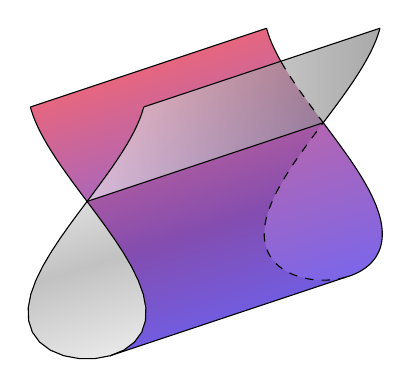
\begin{tikzpicture}[
            declare function  = {
                u(\t) = 3*\t*((\t)^2-1)/(((\t)^2+1)^2);
                v(\t) = 2*((\t)^2-1) / ((\t)^2 + 1);
            }
        ]
            \begin{scope}
                \path[clip]  plot[domain=-0.1:1] ({u(\x)}, {v(\x)}) -- plot[domain=1:-0.1] ({u(\x)+3}, {v(\x)+1}) -- cycle;
                \shade[top color=white, bottom color=white, middle color=black!60!white, shading angle=18, opacity=0.4] (-2,-2) rectangle (4,1);
            \end{scope}
            \begin{scope}
                \path[clip] plot[domain=-1:-0.1] ({u(\x)}, {v(\x)}) -- plot[domain=-0.1:-1] ({u(\x)+3}, {v(\x)+1}) -- cycle;
                \shade[top color=red!60!blue,bottom color=blue,shading angle=18,opacity=0.6] (0,-2) rectangle (4,1);
            \end{scope}
            \begin{scope}
                \path[clip] plot[domain=-1:-2] ({u(\x)}, {v(\x)}) -- plot[domain=-2:-1] ({u(\x)+3}, {v(\x)+1}) -- cycle;
                \shade[bottom color=red!30!blue,top color=red,shading angle=18,opacity=0.6] ({u(-2)},0) rectangle (3,{v(-2)+1});
            \end{scope}
            \begin{scope}
                \path[clip] plot[domain=1:2] ({u(\x)}, {v(\x)}) -- plot[domain=2:1] ({u(\x)+3}, {v(\x)+1}) -- cycle;
                \shade[left color=black!5!white,right color=black!60!white,opacity=0.6] (0,-2) rectangle (4,3);
            \end{scope}

            \draw[black] plot[domain=-2:2, samples=60] ({u(\x)+0}, {v(\x)+0});

            \draw[black] plot[domain=-2:-1.5, samples=60] ({u(\x)+3}, {v(\x)+1});
            \draw[black, dashed] plot[domain=-1.5:-1, samples=60] ({u(\x)+3}, {v(\x)+1});
            \draw[black] plot[domain=-1:-0.1, samples=60] ({u(\x)+3}, {v(\x)+1});
            \draw[black, dashed] plot[domain=-0.1:1, samples=60] ({u(\x)+3}, {v(\x)+1});
            \draw[black] plot[domain=1:2, samples=60] ({u(\x)+3}, {v(\x)+1});

            \draw[black] ({u(-2)}, {v(-2)}) -- ({u(-2)+3}, {v(-2)+1});
            \draw[black] ({u(2)}, {v(2)}) -- ({u(2)+3}, {v(2)+1});
            \draw[black] ({u(1)}, {v(1)}) -- ({u(1)+3}, {v(1)+1});
            \draw[black] ({u(-0.1)}, {v(-0.1)}) -- ({u(-0.1)+3}, {v(-0.1)+1});
        \end{tikzpicture}
    \end{minipage}
    \caption{The sphere ball and the cone (with vertex and base removed) are examples of regular surfaces, while the self-intersecting sheet is not regular surface.}
    \label{fig:diffgeom-surface-examples}
\end{figure}

\begin{defn}
    A subset $S \subseteq \R^3$ is a \emph{regular surface} if for all $p \in S$ there exists a neighborhood $W$ of $p$ (within $\R^3$), an open set $U \subseteq \R^2$, and a map $m: U \to W \intersect S$ such that
    \begin{enumerate}[label=(\roman*)]
        \item $m(u, v) = (x(u, v), y(u, v), z(u, v))$ is a smooth function,
        \item $m$ is a homeomorphism,
        \item the cross-product vector
        \begin{align*}
            \frac{\partial m}{\partial u} \times \frac{\partial m}{\partial v}
        \end{align*}
        is nowhere zero on $U$.
    \end{enumerate}
\end{defn}

\begin{rmk}\proofbreak
    \begin{enumerate}[label=(\roman*)]
        \item allows us to do calculus on surfaces,
        \item prevents self-intersection, and ensures certain properties of $S$ are independent of $W$, $U$, and $m$,
        \item ensures there is a well-defined normal vector to construct a tangent plane.
    \end{enumerate}
\end{rmk}

\begin{defn}
    A mapping $m: U \to W \intersect S$ as defined above is a \emph{local parameterization} of $S$, or a \emph{chart} for $S$. A collection of charts, such that every $p \in S$ is contained in at least one chart, is an \emph{atlas} for $S$.
\end{defn}

\begin{prop}
    The sphere $S^2$ is a regular surface. We will consider $S^2$ as a subset of $\R^3$ given by $\{p \in \R^3 : \norm{p}_2 = 1\}$.

    We will prove a chart exists for all $p \in S^2$. Consider $p \in S^2$ with positive $z$-coordinate. Take $U$ to be the open unit disc $\{u \in \R^2 : \norm{u}_2 < 1\}$, and $W$ the upper half-space $\{(x, y, z) \in \R^3 : z > 0\}$. Define the first chart $m^{(1)}: U \to W \intersect S^2$ by
    \begin{align*}
        m^{(1)}(u, v) &= \left(u, v, \sqrt{1 - (u^2 + v^2)}\right).
    \end{align*}
    This is clearly smooth since $u^2 + v^2 < 1$, and it is a homeomorphism since the inverse of $m^{(1)}$ is $(u, v, w) \mapsto (u, v)$, which is certainly continuous. Finally,
    \begin{align*}
        \frac{\partial m^{(1)}}{\partial u} \times \frac{\partial m^{(1)}}{\partial v} = \begin{pmatrix}
            1, 0, \frac{-u}{\sqrt{1 - (u^2+v^2)}}
        \end{pmatrix} \times \begin{pmatrix}
            0, 1, \frac{-v}{\sqrt{1 - (u^2+v^2)}}
        \end{pmatrix},
    \end{align*}
    which is clearly non-zero since they are linearly independent.

    We can analogously define charts for the bottom, front, top, left, right of the sphere, and so cover the entire sphere with an atlas.
\end{prop}

\begin{exmp}
    The following are examples of atlases for regular surfaces.
    \begin{itemize}
        \item A plane $\{x \in \R^3 : \langle n, x\rangle = c\}$, which can be parameterized with a single chart $m(u, v) = cn/\langle n, n \rangle + us + vt$, where $s, t$ are linearly independent vectors both perpendicular to $n$.
        \item A cut cylinder can be parameterized with the chart $m(u, v) = (a\cos(u), a\sin(u), v)$, where $U = (0, 2\pi) \times (0, 1)$.
        \item An infinite cone (without a vertex) can be parameterized with the chart
        \begin{align*}
            m(u, v) = (av\cos(u), av\sin(u), v),
        \end{align*}
        with $U = (0, 2\pi) \times (0, \infty)$.
        \item A helicoid can be parameterized by the chart $m(u, v) = (av\cos(u), av\sin(u), u)$, where $(u, v) \in (0, 2\pi) \times \R$.
        \item The sphere with a point removed can be parameterized by
        \begin{align*}
            m(u, v) = (\cos(v)\cos(u), \sin(v)\cos(u), \sin(u))
        \end{align*}
        where $(u, v) \in (-\pi/2, \pi/2) \times (0, 2\pi)$.
    \end{itemize}
\end{exmp}

\begin{prop}\label{prop:graph-is-regular-surface}
    Consider a smooth function $f: U \to \R$, where $U \subseteq \R^2$ is open. The graph of $f$ is a regular surface.
\end{prop}

\begin{proof}
    Define $m(u, v) = (u, v, f(u, v))$. Then we will show $m: U \to S$ is a chart for the graph of $f$.

    Smoothness of $m$ follows from the smoothness of $f$. The inverse of $m$ is simply the projection of $\R^3$ onto the $(u, v)$ plane, which is continuous. Finally,
    \begin{align*}
        \frac{\partial m}{\partial u} &= (1, 0, \frac{\partial f}{\partial u}), \\
        \frac{\partial m}{\partial v} &= (0, 1, \frac{\partial f}{\partial v}),
    \end{align*}
    which are trivially linearly independent.
\end{proof}

\begin{defn}
    Suppose $U \subseteq \R^n$ is open, and $F: U \to \R^m$ is smooth. We say that $p \in U$ is a \emph{critical point} of $F$ if $dF_p: \R^n \to \R^m$ fails to be surjective. If $p \in U$ is a critical point, then $F(p) \in \R^m$ is a \emph{critical value} of $F$. A point in $\R^m$ which is \emph{not} a critical value of $F$ is a \emph{regular value} of $F$.
\end{defn}

\begin{thm}
    If $f: U \to \R^3 \to \R$ is smooth, $U$ is open, and $\alpha \in f(U)$ is a regular value, then $f^{-1}(\{\alpha\})$ is a regular surface in $\R^3$.
\end{thm}

\begin{proof}
    Suppose that $p = (x_0, y_0, z_0) \in f^{-1}(\{a\})$. Since $\alpha$ is a regular value of $f$, we know $\nabla f(p) \neq \vec{0}$. Without loss of generality, we will suppose that $\frac{\partial f}{\partial z}(p) \neq 0$. Define $F: U \to \R^3$ by $(x, y, z) \mapsto (x, y, f(x, y, z))$. Then
    \begin{align*}
        dF_{p} = \begin{pmatrix}
            1 & 0 & 0 \\
            0 & 1 & 0 \\
            \frac{\partial f}{\partial x}(p) & \frac{\partial f}{\partial y}(p) & \frac{\partial f}{\partial z}(p)
        \end{pmatrix}.
    \end{align*}
    Since $\frac{\partial f}{\partial z}(p) \neq 0$ by assumption, $dF_p$ must be invertible. By the Inverse Function Theorem \ref{thm:inverse-function}, there exists a neighborhood $V$ of $p$ and $W$ of $F(p)$ such that $F: V \to W$ has smooth inverse $F^{-1}: W \to V$, which necessarily has the form $F^{-1}(u, v, w) = (u, v, g(u, v, w))$ for some smooth $g: W \to \R$. Next, we can define $h: \tilde{W} \to V$ by $h(u, v) = g(u, v, \alpha)$, where $\tilde{W}$ is the projection of $W$ onto the $UV$ plane.
    
    Notice that the graph of $h$ is $f^{-1}(\{\alpha\}) \intersect V$. By Proposition \ref{prop:graph-is-regular-surface}, $h$ is a chart for $p$, and so $f^{-1}(\{\alpha\})$ must be a regular surface.
\end{proof}

\begin{cor}
    Taking $f(p) = \norm{p}_2$, we have that $S^2$ is a regular surface since $S^2 = f^{-1}(\{1\})$ and $S^2$ doesn't include $0$, which is the only critical value of $f$.
\end{cor}

\begin{thm}
    Given $S \subseteq \R^3$ be a regular surface. For any $p \in S$, there exists a neighborhood $V$ of $p$ such that $V$ is the graph of a smooth function whose form is either $z = f(x, y)$, $y = g(x, z)$, or $x = h(y, z)$.
\end{thm}

\begin{lemma}\label{lemma:change-of-chart}
    Suppose that $S$ is a regular surface and $p \in S$. Suppose that $x: U \to S$ and $y: V \to S$ are two charts of $p$. Take $\Omega = x(U) \intersect y(V)$. Then
    \begin{align*}
        h&: y^{-1}(\Omega) \to x^{-1}(\Omega), \\
        h&: (u, v) \mapsto x^{-1}(y(u, v))
    \end{align*}
    is a diffeomorphism.
\end{lemma}

\begin{proof}
    Since $x$ and $y$ are homeomorphisms by the definition of a chart, so is $h = x^{-1} \circ y$. Now fix arbitrary $r \in y^{-1}(\Omega)$, and let $q = h(r) \in x^{-1}(\Omega)$. Since $dx(q)$ and $dy(r)$ must both be injective by the third condition of the definition of a chart, it follows there is a unit vector $w$ in the orthogonal complement of the image of $dx(q)$.

    Define $F: U \times R \to \R^3$ by $F(u, v, t) = x(u, v) + tw$. Since $x$ is smooth, so is $F$. Furthermore,
    \begin{align*}
        dF(q, t) = dx(q) + tw
    \end{align*}
    must be full-rank, since $dx(q)$ is injective and $w$ is orthogonal to its image. Therefore, we can apply the inverse function theorem \ref{thm:inverse-function} to find that $F$ is a diffeomorphism in some neighborhood $M$ of $(q, 0)$. Therefore, $h = \pi \circ F^{-1} \circ y$ (where $\pi$ is the projection onto the $uv$ plane) is smooth in a neighborhood of $r$.

    Since the roles of $x$ and $y$ are symmetric, interchanging them yields smoothness of $y^{-1} \circ x = h^{-1}$.
\end{proof}

\begin{defn}
    Let $S$ be a regular surface, and let $f: S \to \R$. Given a point $p \in S$, let $m(u, v): U \to S$ be a chart at $p$. Then $f$ is smooth at $p$ when $f \circ m$ is smooth at $m^{-1}(p)$. We say $f$ is smooth if it is smooth at all $p \in S$.
\end{defn}

\begin{lemma}
    A function $f: S \to \R$ is smooth at a point $p$, independent of the choice of chart used. That is, if it is smooth with respect to one chart then it is smooth with respect to every chart, and conversely if it is not smooth with respect to one chart then it is not smooth with respect to any chart.
\end{lemma}

\begin{proof}
    Suppose $f: S \to \R$ is smooth at $p \in S$ with respect to a chart $x: U \to \R$, and consider another chart $y: V \to \R$, such that $p \in U \intersect V = \Omega$. But then $f \circ y = (f \circ x) \circ (x^{-1} \circ y)$. Since $f \circ x$ and $x^{-1} \circ y$ are both diffeomorphisms by assumption and by Lemma \ref{lemma:change-of-chart} respectively, $f \circ y$ must be smooth.
\end{proof}

\begin{rmk}
    We have defined the notion of a smooth function from $S \to \R$, however we can just as easily define the smoothness of a function between regular surfaces.
\end{rmk}

\begin{defn}
    Let $S_1$ and $S_2$ be regular surfaces, and consider a \emph{continuous} function $f: S_1 \to S_2$. Consider a point $p \in S_1$ and parameterizations $x: U_1 \subseteq \R^2 \to S_1$ and $y: U_2 \subseteq \R^2 \to S_2$ such that $p \in x(U_1)$ and $f(x(U_1)) \subseteq y(U_2)$. We say $f$ is smooth at $p$ if $y^{-1} \circ f \circ x: U_1 \to U_2$ is smooth at $x^{-1}(p)$.
\end{defn}

\begin{prop}
    Lemma \ref{lemma:change-of-chart} again tells us this definition is independent of the particular atlas/charts used to prove smoothness of $f$.
\end{prop}

\begin{defn}
    We say two regular surfaces $S_1$ and $S_2$ are \emph{diffeomorphic} if there exists a smooth function $f: S_1 \to S_2$ with smooth inverse.
\end{defn}

\begin{prop}
    Let $x: U \subseteq \R^2 \to S$ be a mapping satisfying the first and third conditions of the definition of a local parameterization. If $x$ is injective, then $f$ has a continuous inverse and so is a local parameterization.
\end{prop}

\begin{proof}
    {\Large\color{red}TODO: find in do Carmo}
\end{proof}

\section{Tangent planes and differentials}

\begin{defn}
    Let $S \subseteq \R^3$ be a regular surface. A vector $v$ is a \emph{tangent vector} to $p \in S$ if there exists a smooth curve $\alpha: (-\varepsilon, \varepsilon) \to S$ such that $\alpha(0) = p$ and $\alpha'(0) = v$.
\end{defn}

\begin{defn}
    Let $S \subseteq \R^3$ be a regular surface, and $p \in S$. The \emph{tangent plane} of $S$ at $p$ is the set of tangent vectors to $S$ passing through $p$, and is denoted by $T_pS$.
\end{defn}

\begin{prop}
    Let $x: U \to S$ be a local parameterization of a regular surface $S$, and let $q \in U$. Then $dx_q$ is a linear isomorphism between vectors in $\R^2$ and the tangent plane at $p$.
\end{prop}

\begin{proof}
    Let $w$ be a tangent vector to $S$ at $x(q)$, so $w = \alpha'(0)$ for some smooth curve $\alpha: (-\varepsilon, \varepsilon) \to S$, with $\alpha(0) = x(q)$. In particular, for $\varepsilon$ small enough, $x$ is a local parameterization for all points in the trace of $\alpha$. Therefore, we consider the curve $\beta = x^{-1} \circ \alpha$. Therefore, $dx_q(\beta'(0)) = \alpha'(0)$ by definition of $dx_q$.

    Conversely, consider any $w = dx_q(v)$ for $v \in \R^2$. Then consider the curve $\beta(t) = q + tv$, and define $\alpha = x \circ \beta$. Then $\alpha(0) = x(q)$, and $\alpha'(0) = dx_q(\beta'(0)) = dx_q(v) = w$. Therefore $w$ is a tangent vector at $x(q)$.

    It follows that the range of $dx_q$ is the set of tangent vectors of $S$ at $x(q)$. Since $dx_q$ is injective by definition of a chart, it follows that $dx_q$ is a bijection between $\R^2$ and the set of tangent vectors.
\end{proof}

\begin{cor}
    Therefore, the tangent plane is a vector space over $\R$.
\end{cor}

\begin{defn}
    Let $S_1$ and $S_2$ be regular surfaces, and suppose $\varphi: V \subseteq S_1 \to S_2$ is smooth, where $V$ is open. Let $p \in V$ and define $d\varphi_p: T_pS_1 \to T_{\varphi(p)}S_2$ by $d\varphi_p(w) = \beta'(0)$, where $\beta = \varphi \cdot \alpha$, and $\alpha: (-\varepsilon, \varepsilon) \to S_1$ is such that $w = \alpha'(0)$ and $\alpha(0) = p$. The map $d\varphi_p$ is the \emph{differential} of $\varphi$ at $p$.
\end{defn}

\begin{prop}
    Despite the apparent dependence of the above definition on exactly which $\alpha$ is chosen to represent the tangent vector $\alpha'(0)$, the definition is well-defined and independent of this choice.
\end{prop}

\begin{proof}
    Let $g: \R^2 \to S_1$ be a local parameterization at $p$, and let $h: \R^2 \to S_2$ be a local parameterization at $\varphi(p)$. Therefore, we can express $\varphi: \R^2 \to \R^2$ with respect to these parameterizations as
    \begin{align*}
        \varphi(u, v) = (\varphi_1(u, v), \varphi_2(u, v)),
    \end{align*}
    and $\alpha(t) = (u(t), v(t))$ for $t \in (-\varepsilon, \varepsilon)$. Therefore,
    \begin{align*}
        \beta(t) &= \varphi(\alpha(t)) = \varphi(u(t), v(t)) = \left(\varphi_1(u(t), v(t)), \varphi_2(u(t), v(t))\right).
    \end{align*}
    Therefore, in the basis defined at $\varphi(p)$ by $dh(p)$, we have
    \begin{align*}
        \beta'(0) &= \left(\frac{\partial \varphi_1}{\partial u}\frac{\partial u}{\partial t}(0) + \frac{\partial \varphi_1}{\partial v}\frac{\partial v}{\partial t}(0), \frac{\partial \varphi_2}{\partial u}\frac{\partial u}{\partial t}(0) + \frac{\partial \varphi_2}{\partial v}\frac{\partial v}{\partial t}(0)\right).
    \end{align*}
    Since the partial derivatives of $\varphi_1, \varphi_2$ with respect to $u, v$ are dependent only on $\varphi$ itself, and the derivatives $u'(0)$ and $v'(0)$ depend only on $w$, not on $\alpha$, it follows that $d\varphi_p$ is well-defined.
\end{proof}

\begin{rmk}
    With respect to the bases imposed by $h$ and $g$, it follows that
    \begin{align*}
        d\varphi_p = \begin{bmatrix}
            \dfrac{\partial \varphi_1}{\partial u} & \dfrac{\partial \varphi_1}{\partial v} \\
            \dfrac{\partial \varphi_2}{\partial u} & \dfrac{\partial \varphi_2}{\partial v}
        \end{bmatrix}.
    \end{align*}
\end{rmk}

\section{First Fundamental Form}

\begin{defn}
    Let $S \subseteq \R^3$ be a regular surface, and let $p \in S$. The \emph{first fundamental form} of $S$ at $p$ is the map $\ffform_p: T_pS \to \R$ defined by $\ffform_p(w) = \norm{w}_2^2$.
\end{defn}

\begin{prop}
    Given a local parameterization $m: \R^2 \to S$, there exist $E, F, G \in \R$ such that the following holds: for any $w \in T_pS$ and $\alpha: (-\varepsilon, \varepsilon) \to S$ such that $\alpha(t) = (u(t), v(t))$ and $w = \alpha'(0)$, we can express $\ffform_p(w)$ as the quadratic form
    \begin{align*}
        \ffform_p(w) &= Eu'(0)^2 + Fu'(0)v'(0) + Gv'(0)^2.
    \end{align*}
\end{prop}

\begin{proof}
    The first fundamental form is given by $\ffform_p(w) = \ffform_p(\alpha'(0))$, so
    \begin{align*}
        \ffform_p(w) &= \langle \alpha'(0), \alpha'(0) \rangle \\
        &= \left\langle \frac{\partial m}{\partial u}u'(0) + \frac{\partial m}{\partial v}v'(0), \frac{\partial m}{\partial u}(p)u'(0) + \frac{\partial m}{\partial v}(p)v'(0) \right\rangle \\
        &= u'(0)^2\left\langle \frac{\partial m}{\partial u}(p), \frac{\partial m}{\partial u}(p) \right\rangle + v'(0)^2\left\langle \frac{\partial m}{\partial v}(p), \frac{\partial m}{\partial v}(p) \right\rangle + u'(0)v'(0)\left\langle \frac{\partial m}{\partial u}(p), \frac{\partial m}{\partial v}(p) \right\rangle \\
        &= Eu'(0)^2 + 2Fu'(0)v'(0) + Gv'(0)^2 \\
        &= \begin{pmatrix}
            u'(0) \\ v'(0)
        \end{pmatrix}^{\transpose}\begin{pmatrix}
            E & F \\ F & G
        \end{pmatrix}\begin{pmatrix}
            u'(0) \\ v'(0)
        \end{pmatrix}.
    \end{align*}
\end{proof}

\begin{exmp}
    Consider a surface of revolution with unit speed profile curve $\gamma(t) = (f(t), 0, g(t))$, such that $f$ is positive and $\gamma$ does not self-intersect. The surface of revolution is then parameterized by $m(u, v) = (f(u)\cos(v), f(u)\sin(v), g(u))$. The first fundamental form with respect to $m$ is therefore given by
    \begin{align*}
        E &= \norm{\frac{\partial m}{\partial u}(p)}_2^2 = \norm{(f'(u)\cos(v), f'(u)\sin(v), g'(u))}^2 = f'(u)^2 + g'(u)^2 = 1 \\
        F &= \left\langle \frac{\partial m}{\partial u}(p), \frac{\partial m}{\partial v}(p) \right\rangle = 0 \\
        G &= \norm{\frac{\partial m}{\partial v}(p)} = f^2(u).
    \end{align*}
\end{exmp}

\begin{rmk}
    We can also use the fundamental form matrix to compute angles between tangent curves at a point $p$.
\end{rmk}

\begin{defn}
    Let $S$ be a regular surface, and $\alpha: I \to S$ and $\beta: I \to S$ to be two parameterized curves such that $\alpha(t_0) = \beta(t_0)$. Then the angle between then at $\alpha(t_0)$ is given by
    \begin{align*}
        \cos(\theta) &= \frac{\langle \alpha'(t_0), \beta'(t_0) \rangle}{\norm{\alpha'(t_0)}\norm{\beta'(t_0)}}.
    \end{align*}
\end{defn}

\begin{lemma}
    With respect to a local parameterization $m: U \to S$ of $p \in S$, the angle between curves $\alpha, \beta: I \to S$ such that $\alpha(t_0) = p = \beta(t_0)$ is such that
    \begin{align*}
        \cos(\theta) = \frac{w^{\transpose}Mv}{\sqrt{w^{\transpose}Mw}\sqrt{v^{\transpose}Mv}},
    \end{align*}
    where $w = d(m^{-1} \circ \alpha)$, $v = d(m^{-1} \circ \beta)$, and $M$ is the matrix representation of the first fundamental form at $p$:
    \begin{align*}
        M = \begin{pmatrix}
            E & F \\ F & G
        \end{pmatrix}.
    \end{align*}
\end{lemma}

\begin{rmk}
    If $w = (1, 0)$ and $v = (0, 1)$, the $\cos(\theta) = F/\sqrt{EG}$.
\end{rmk}

\begin{defn}
    Let $R \subseteq S \subseteq \R^3$ be a region of a regular surface, such that all of $R$ lies within one local parameterized $m: U \to S$. Then the \emph{area} of $R$ is defined to be
    \begin{align*}
        A(R) &= \iint_{m^{-1}(R)}\norm{m_u \times m_v}dudv.
    \end{align*}
\end{defn}

\begin{prop}
    The area of a region is independent of the parameterization used.
\end{prop}

\begin{rmk}
    Note that
    \begin{align*}
        \norm{m_u \times m_v}^2 &= \norm{m_u}^2\norm{m_v}^2 - \left(\langle m_u, m_v \rangle\right)^2 \\
        &= EG - F^2,
    \end{align*}
    and so $\norm{m_u \times m_v} = \sqrt{EG-F^2}$, which is the square root of the determinant.
\end{rmk}

\begin{rmk}
    Recall that a surface of revolution with profile curve $\gamma(u) = (f(u), 0, g(u))$ will have local parameterization $m(u, v) = (f(u)\cos(v), f(u)\sin(v), g(u))$ for $v \in (0, 2\pi)$.

    Consider the torus, described as a circle of revolution with profile curve given by $f(u) = 2 + \cos(u)$ and $g(u) = \sin(u)$ for $u \in (0, 2\pi)$. Therefore, the local parameterization is
    \begin{align*}
        m(u, v) = (\cos(v)(2 + \cos(u)), \sin(v)(2 + \cos(u)), \sin(u)),
    \end{align*}
    and we have
    \begin{align*}
        \frac{\partial m}{\partial u} &= (-\sin(u)\cos(u), -\sin(u)\sin(v), \cos(u)), \\
        \frac{\partial m}{\partial v} &= (-\sin(v)(2 + \cos(u)), \cos(v)(2 + \cos(u)), 0).
    \end{align*}
    Therefore, the first fundamental form is represented by
    \begin{align*}
        E &= \norm{m_u}^2 = 1, \\
        F &= 0, \\
        G &= (2 + \cos(u))^2,
    \end{align*}
    and so the torus has area given by
    \begin{align*}
        \int_{0}^{2\pi}\int_{0}^{2\pi}\abs{2 + \cos(u)}dudv = \int_{0}^{2\pi}(4\pi + 0)dv = 8\pi^2.
    \end{align*}
\end{rmk}

\section{Orientation}

\begin{defn}
    For a regular surface $S$, we say that $n \in \R^3$ is \emph{normal} to $S$ at $p$ if $n$ is in the orthogonal complement of $TpS$.
\end{defn}

\begin{defn}
    Let $S \subseteq \R^3$ be a regular surface, and let $R$ be an open subset of $S$. A smooth unit normal vector field on $R$ is a smooth map $N: R \to \R^3$ such that $N(p)$ is normal to $S$ and $\norm{N(p)} = 1$ for all $p \in R$.
\end{defn}

\begin{defn}
    A regular surface $S$ is \emph{orientable} if there exists a smooth unit normal vector field on all of $S$.
\end{defn}

\begin{exmp}
    The M\"obius strip (shown in Figure \ref{fig:mobius}) is a non-orientable regular surface.

    \begin{figure}
        \centering
        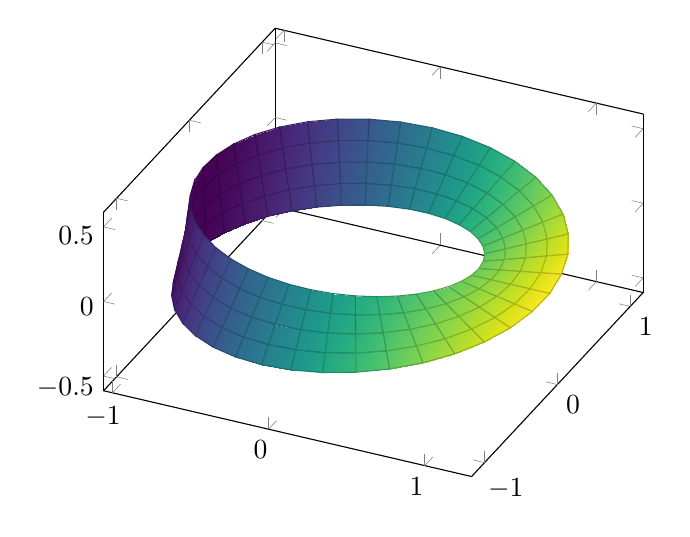
\begin{tikzpicture}
            \centering
            \begin{axis}[
                unit vector ratio=1 1 1
            ]
                \addplot3 [
                    surf, shader=faceted interp,
                    point meta=x,
                    colormap/viridis,
                    samples=40,
                    samples y=5,
                    z buffer=sort,
                    domain=0:360,
                    y domain=-0.5:0.5
                ] (
                    {(1+0.5*y*cos(x/2))*cos(x)},
                    {(1+0.5*y*cos(x/2))*sin(x)},
                    {0.5*y*sin(x/2)});
            \end{axis}
        \end{tikzpicture}
    \caption{M\"obius surface}
    \label{fig:mobius}
    \end{figure}
\end{exmp}

\begin{rmk}
    Given a local parameterization $m: U \subseteq \R^2 \to S$, then one unit normal vector at $p \in m(U)$ is given by
    \begin{align*}
        N(p) = \frac{m_u \times m_v}{\norm{m_u \times m_v}},
    \end{align*}
    where $m_u$ and $m_v$ are the partials derivatives of $m$. Note that $-N(p)$ is also a unit normal vector $p$. Since $TpS$ is independent of any local parameterization, so is $\pm N(p)$ (up to sign). Furthermore, since charts are smooth, so is the unit normal.
\end{rmk}

\begin{thm}\label{thm:orientable-atlas}
    A regular surface $S$ is orientable if and only if there exists an atlas $\{m_i: U_i \subseteq \R^n \to S\}$ such that for any $m_i(u_i, v_i), m_j(u_j, v_j)$, the transition map
    \begin{align*}
        \frac{\partial (u_i, v_i)}{\partial (u_,v_j)} = \begin{pmatrix}
            \frac{\partial u_i}{\partial u_j} & \frac{\partial u_i}{\partial v_j} \\
            \frac{\partial v_i}{\partial u_j} & \frac{\partial v_i}{\partial v_j}
        \end{pmatrix}
    \end{align*}
    has positive determinant at all $p \in m_i(U_i) \intersect m_j(U_j)$.
\end{thm}

\begin{proof}
    If $m: U \to S$ and $w: V \to S$ are two local parameterizations such that $p \in m(U) \intersect w(V)$, then $m_u \times m_v = \frac{\partial (u,v)}{\partial (a, b)}(w_a \times w_b)$. Therefore, the unit normals defined by distinct overlapping charts are the same if and only if the transition map has strictly positive determinant.
\end{proof}

\begin{cor}
    If a surface has a global parameterization, then it is orientable.
\end{cor}

\begin{prop}
    If a regular surface $S$ can be covered by two charts $m: U \to S$ and $w: V \to S$ such that $m(U) \intersect w(V)$ is connected, then $S$ is orientable.
\end{prop}

\begin{proof}
    The determinant of the transition map is continuous and non-zero, so it must be positive on all of $m(U) \intersect w(V)$, or negative on all of $m(U) \intersect w(V)$. If it is positive, then by Theorem \ref{thm:orientable-atlas} we are done. Otherwise, we replace the chart $w$ with $q(u, v) = w(u, v)$. Then $q$ is still a chart, with the same image (although a different domain), but the rows of the transition map are swapped, and therefore the determinant of the transition map is now positive.
\end{proof}

\begin{prop}
    Let $S$ be a regular surface defined by $S = f^{-1}(\{a\})$ for some $f: \R^3 \to \R$, where $f$ is smooth and $a$ is a regular value of $f$. Then $S$ is orientable.
\end{prop}

\begin{proof}
    Since $\nabla f(p)$ doesn't vanish on $S$, we know that $\nabla f(p)/\norm{\nabla f(p)}$ defines a unit normal for all $p \in S$. Since $f$ is smooth, so is $\nabla f$, and so this unit normal vector field is smooth.
\end{proof}

\begin{thm}\label{thm:orientable-preserved-diffeomorphism}
    Let $S_1$ and $S_2$ be regular surfaces, and let $\varphi: S_1 \to S_2$ be a diffeomorphism. Then $S_1$ is orientable if and only if $S_2$ is orientable.
\end{thm}

\begin{proof}
    For any $p \in S_1$, let $m: U \subseteq \R^2 \to S_1$ be a chart for $p$ and $w: V \subseteq \R^2 \to S_2$ be a chart for $\varphi(p)$. Since $\varphi$ is a diffeomorphism, we know that $\psi = w^{-1} \circ \varphi \circ m$, where $\psi: U \to V$, must be a diffeomorphism. Then $\gamma = \varphi \circ m = w \circ \psi$ is a chart for $\varphi(U) \in S_2$. This is because
    \begin{itemize}
        \item $\gamma$ is the composition of smooth functions, and therefore is smooth,
        \item $\gamma$ is the composition of homeomorphisms, and therefore is a homeomorphism,
        \item and $dm$ is injective since $m$ is a chart, and $d\varphi$ is bijective since $\varphi$ is a diffeomorphism, so $d\gamma = d(\varphi \circ m) = (d\varphi)(dm)$ is injective.
    \end{itemize}

    Suppose that $S_1$ is orientable. Then by Theorem \ref{thm:orientable-atlas} there exists an atlas $A_1$ for $S_1$ such that every transition map between charts has positive determinant. Let $B = \{ \varphi \circ m : m \in A \}$. We just proved that $B$ is a set of charts for $S_2$. For any point $p \in S_2$, we know $\varphi^{-1} \in S_1$ has a chart $m \in A$. Then $\varphi \circ m$ contains $p$ in its domain, and so $B$ is in fact an atlas for $S_2$.

    Now, notice the following relation between transition maps. For any $w_1, w_2 \in B$, by construction there exist $m_1, m_2 \in A$ such that $w_1 = \varphi \circ m_1$ and $w_2 = \varphi \circ m_2$. Letting $H$ be the intersection of the images of $w_1$ and $w_2$, we have at points in $H$ that
    \begin{align*}
        \frac{\partial w_1}{\partial w_2} = d\left(w_1^{-1} \circ w_2\right) = d(m_1^{-1} \circ \varphi^{-1} \circ \varphi \circ m_2) = d(m_1^{-1} \circ m_2) = \frac{\partial m_1}{\partial m_1}.
    \end{align*}
    By our choice of atlas $A$, we know that the transition map between $m_1$ and $m_2$ has positive determinant, so this proves that the transition map between $w_1$ and $w_2$ does as well. Therefore, by Theorem \ref{thm:orientable-atlas} we know that $S_2$ is orientable.

    The converse follows immediately from symmetry of $S_1$ and $S_2$.
\end{proof}

\section{Gauss map}

\begin{defn}
    Let $S$ be an orientable surface. A smooth unit normal vector field $N$ on $S$ is an \emph{orientation} of $S$.
\end{defn}

\begin{defn}
    Let $S$ be a regular surface with orientation $N$. The \emph{Gauss map} is the map $p \mapsto N(p)$ from $S \to S^2$ (the unit sphere).
\end{defn}

\begin{rmk}
    Consider the differential of the Gauss map $dN(p): T_pS \to T_{N(p)}S^2$, and notice that since $T_pS$ and $T_{N(p)}S^2$ have the same normal vector (by construction of the Gauss map), we can identify these vectors space. Therefore, we will consider the differential of the Gauss map to be a map $dN(p): T_pS \to T_pS$.
\end{rmk}

\begin{rmk}
    For a curve $\alpha: I \to S$, let $N(t)$ be short for $N(\alpha(t))$. Then $N'(0) = dN_{\alpha(0)}(\alpha'(0))$, so $N'(0)$ can be interpreted as measuring the rate of change of the normal vectors along $\alpha$ at $p$. 
\end{rmk}

\begin{exmp}
    Consider the unit sphere, with inward orientation. That is,
    \begin{align*}
        N(x,y,x) = -(x,y,z).
    \end{align*}
    For $p \in S$ and a curve $\alpha$ such that $\alpha(0) = p$, we have
    \begin{align*}
        dN_p(\alpha'(0)) &= \frac{d}{dt}|_{t=0}(-x(t), -y(t), -z(t)) = -\alpha'(0).
    \end{align*}
\end{exmp}

\begin{defn}
    The \emph{second fundamental form} of a regular surface $S$ at $p \in S$ is the map $\sfform_p: T_pS \to \R$ given by $\sfform_p(v) = -\langle dN_p(v), v\rangle$.
\end{defn}

\begin{defn}
    Let $S$ be a regular surface with orientation $N$, and let $c \subseteq S$ be a regular parameterized curve passing through some $p \in S$. Let $\kappa$ be the curvature of $c$ at $p$, let $n(p)$ be the normal vector of $c$, and $N(p)$ the normal vector of $S$. Define $\cos(\theta) = \langle n(p), N(p) \rangle$, and then the \emph{normal curvature} of $C$ at $p$ in $S$ is $\kappa\cos(\theta)$. If $\kappa = 0$, so the normal $n(p)$ is not defined, then we define the normal curvature to be zero. We denote the normal curvature at $p$ by $\kappa_n(p)$.
\end{defn}

\begin{prop}
    Let $v \in T_pS$. The normal curvature of any curve $C$ with tangent vector $v$ at $p$ is independent of $C$, and is equal to $\sfform_p(v)$.
\end{prop}

\begin{proof}
    Suppose $\alpha = \alpha(s)$ is a unit speed parameterization of $C$, such that $\alpha(0) = p$ and $\alpha'(0) = v$. Let $N(s)$ be the normal vector of the surface at $\alpha(S)$. Since $\alpha'(s) \in T_{\alpha(s)}S$, we know that
    \begin{align*}
        \langle N(s), \alpha'(s)\rangle = 0,
    \end{align*}
    and so differentiating we obtain
    \begin{align*}
        \langle N'(s), \alpha'(s)\rangle = -\langle N(s), \alpha''(s)\rangle.
    \end{align*}
    Therefore, the second fundamental form at $p$ is given by
    \begin{align*}
        \sfform_{p}(v) &= -\langle dN_p(\alpha'(s)), \alpha'(0)\rangle = -\langle N'(0), \alpha'(0)\rangle = \langle N(0), \alpha''(0)\rangle.
    \end{align*}
    By Frenet-Serret, since $\alpha$ is unit speed we have $\alpha''(0) = \kappa(p)n(p)$, and so
    \begin{align*}
        \sfform_p(v) = \kappa(p)\langle N(p), n(p)\rangle = \kappa_n(p).
    \end{align*}
\end{proof}

\begin{rmk}
    Since the normal curvature is independent of the curve used, for convienence we can always use the plane formed by the intersection of $S$ with the plane spanned by $N(p)$ and $v$. This curve is known as the \emph{normal section} of $S$ at $p$, along $v$.
\end{rmk}

\begin{exmp}
    For the plane, all normal sections are straight lines, and so the normal curvature is zero everywhere.

    For the unit sphere, with inward orientation, the normal sections are great circles. Therefore, the normal vector of any normal section is equal to the normal vector of the surface. Therefore, the normal curvature is $\kappa_n(p) = \kappa(p)1 = 1$, since a unit circle has curvature $1$.

    For a unit cylinder with inward orientation, the normal section depends on the parameterization used. We can choose a parameterization such that the normal section is a circle, giving $\kappa_n(p) = 1$, or by swapping $(u, v)$ we get a normal section equal to a line, so $\kappa_n(p) = 0$.
\end{exmp}

\begin{defn}
    Let $S$ be a regular surface, and $p \in S$. The maximum and minimum normal curvatures of $S$ at $p$, denoted by $\kappa_1(p), \kappa_2(p)$ are called the \emph{principal curvatures} of $S$ and $p$. A unit vector which attain these extrema is called a \emph{principal direction}.
\end{defn}

\begin{defn}
    For a plane or sphere, $\kappa_1(p) = \kappa_2(p)$, so all directions are principal directions.

    For the cylinder with inward orientation, $\kappa_1(p) = 1$ and $\kappa_2(p) = 0$, with corresponding principal directions $p \times w$ and $w$, where $w$ is the cylinder's axis.
\end{defn}

\begin{thm}\label{thm:principal-directions-gauss-eigenvectors}
    Let $S$ be a regular surface. For $p \in S$, let $v_1(p), v_2(p)$ be principal directions corresponding to $\kappa_1(p)$ and $\kappa_2(p)$. Then $\{v_1(p), v_2(p)\}$ forms an orthonormal basis for $T_pS$, and $-dN_p(v_1) = \kappa_1v_1$ and $-dN_p(v_2) = \kappa_2v_2$.
\end{thm}

\begin{proof}
    Since $dN_{p}: T_pS \to T_pS$ is a differential, it is a linear map. Let $m(u, v)$ be a local parameterization for $p \in S$. Then $m_{u}$ and $m_{v}$ form a basis for $T_pS$. Let $\alpha'(0) \in TpS$ be a tangent vector, where $\alpha(t) = m(u(t), v(t))$ for some $u(t), v(t): I \to \R$, $\alpha(0) = p$, and $\alpha$ is unit speed.
    
    Let $N_u = dN_{p}(m_u)$, and $N_v = dN_{p}(m_v)$. We know that $\langle N(p), m_u \rangle = 0$ and $\langle N(p), m_v\rangle = 0$ since $N(p)$ is normal to the tangent plane, so by differentiating with respect to $v$ and $u$ respectively, we obtain
    \begin{align*}
        \langle N_v, m_u \rangle + \langle N(p), m_{uv}\rangle &= 0, \\
        \langle N_u, m_v \rangle + \langle N(p), m_{vu}\rangle &= 0.
    \end{align*}
    Since all second partial derivatives of $m$ are continuous by smoothness of $m$, we know that $m_{uv} = m_{vu}$, and so we have $\langle N_v, m_u\rangle = \langle N_u, m_v \rangle$. Since $N_u = dN_{p}(m_u)$ and $N_v = dN_{p}(m_v)$, it follows that
    \begin{align*}
        \langle dN_{p}(m_u), m_v \rangle = \langle m_u, dN_{p}m_v\rangle.
    \end{align*}
    Therefore, $-dN_{p}$ is self-adjoint, and so by the Spectral Theorem \ref{spectral-theorem} we know that there exists a orthonormal basis of eigenvalues. Furthermore, by the Rayleigh-Ritz theorem \ref{thm:rayleigh-ritz} it follows that the eigenvalues are the principal curvatures of $S$ at $p$, and the corresponding unit eigenvectors are the corresponding principal directions.
\end{proof}

\begin{thm}{Euler's formula}\proofbreak
    For any $v \in TpS$, $\sfform_p(v) = \kappa_1\cos^2(\theta) + \kappa_2\sin^2(\theta)$, where $\theta$ is the angle of $v$, measured from $v_1$ towards $v_2$.
\end{thm}

\begin{proof}
    Since $v_1, v_2$ are an orthonormal eigenbasis, we know that $v = \cos(\theta)v_1 + \sin(\theta)v_2$. Therefore,
    \begin{align*}
        \sfform_p(v) &= \langle -dN_p(\cos(\theta)v_1 + \sin(\theta)v_2), \cos(\theta)v_1 + \sin(\theta)v_2 \rangle \\
        &= \langle \kappa_1\cos(\theta)v_1 + \kappa_2\sin(\theta)v_2, \cos(\theta)v_1 + \sin(\theta)v_2 \rangle \\
        &= \kappa_1\cos^2(\theta) + \kappa_2\sin^2(\theta).
    \end{align*}
\end{proof}

\begin{defn}
    For $p \in S$, the determinant of $-dN_p$ (which is $\kappa_1\kappa_2$) is the \emph{Gauss curvature} $K(p)$ of $S$ at $p$. Additionally, $\frac{1}{2}\trace(-dN_p) = (\kappa_1 + \kappa_2)/2$ is the \emph{mean curvature} $H(p)$ of $S$ at $p$.
\end{defn}

\begin{rmk}
    When we reverse the orientation of $S$, then the sign of $\kappa_1$ and $\kappa_2$ reverse. Therefore, the Gauss curvature $K$ is independent of orientation, but the mean curvature $H$ is not.
\end{rmk}

\begin{defn}
    We say that $p \in S$ is
    \begin{itemize}
        \item \emph{elliptic} when $K(p) > 0$ (e.g. points on surface of a sphere),
        \item \emph{hyperbolic} when $K(p) < 0$ (e.g. points on surface of a hyperbolic paraboloid).
        \item \emph{parabolic} when $K(p) = 0$ but $H(p) \neq 0$ (e.g. points on surface of a cylinder),
        \item \emph{planar} when $K(p) = 0$ and $H(p) = 0$ (e.g. points on surface of a plane).
    \end{itemize}
\end{defn}

\begin{rmk}
    All points in a sufficiently small neighborhood of a elliptic (respectively hyperbolic) point remain elliptic (respectively hyperbolic), by continuity of $K(p)$. However, this is not necessarily the case for parabolic or planar points.
\end{rmk}

\begin{exmp}\proofbreak
    \begin{itemize}
        \item If $S$ is the graph of $z = x^2 + y^2$, all points are elliptic.
        \item If $S$ is the graph of $z = x^4 + y^2$, the origin is a parabolic point, and all other points are elliptic.
        \item If $S$ is the graph of $z = x^4 + y^4$, the origin is planar, and all other points are elliptic. 
    \end{itemize}
\end{exmp}

\begin{defn}
    If $p \in S$ satisfies $\kappa_1(p) = \kappa_2(p)$, then $p$ is an \emph{umbilical point.}
\end{defn}

\begin{exmp}\proofbreak
    \begin{itemize}
        \item Every point on a plane is an umbilical point.
        \item No point on a cylinder is an umbilical point,
        \item On a paraboloid, the origin is the only umbilical point.
    \end{itemize}
\end{exmp}

\begin{prop}
    Let $S$ be a connected surface such that every point $p \in S$ is an umbilical point. Then $S$ is either a portion of a sphere, or a portion of a plane.
\end{prop}

\begin{proof}
    Let $p \in S$, and let $m(u, v)$ be a chart whose image contains $p$. Since every $q \in V$ is umbilical, we have $dN_{q}(w) = \lambda(q)w$, where $\lambda: V \to \R$ is smooth. In fact, $\lambda(q)$ is constant! This is because we can express $w = a_1m_u + a_2m_v$, and so
    \begin{align*}
        dN_q(w) = a_1N_u + a_2N_v,
    \end{align*}
    and then since $dN_q(m_u) = N_u$ and $dN_q(m_v) = N_v$, so $N_u = \lambda(q)m_u$ and $N_v = \lambda(q)m_v$. Differentiating this last two equations with respect to $v$ and $u$ respectively, we obtain $N_{uv} = \lambda_v(q)m_u + \lambda(q)m_{uv}$ and $N_{vu} = \lambda_u(q)m_v + \lambda(q)m_{vu}$. By smoothness, $N_{uv} = N_{vu}$ and $m_{uv} = m_{vu}$, so we have $\lambda_vm_u - \lambda_um_v = \vec{0}$. But $m_u$ and $m_v$ are linearly independent, so it follows that $\lambda_u, \lambda_v$ are zero. Therefore, $\lambda$ is constant as claimed.

    Now we separately consider the cases $\lambda = 0$ and $\lambda \neq 0$. When $\lambda = 0$, we have $N_u = \lambda(q)m_u = \vec{0}$ and similarly $N_v = \vec{0}$. Therefore, $N(q)$ is some constant $N_0$ across the surface. Furthermore,
    \begin{align*}
        \frac{\partial}{\partial u}\langle m, N_0\rangle &= \langle m_u, N_0\rangle + \langle m, \vec{0}\rangle, \\
        \frac{\partial}{\partial v}\langle m, N_0\rangle &= \langle m_v, N_0\rangle + \langle m, \vec{0}\rangle.
    \end{align*}
    Since $N$ is normal to $m_u$ and $m_v$ by definition, it follows that $\langle m(u, v), N(m(u, v))\rangle = \langle q, N(q)\rangle$ is constant, which is precisely the definition of a plane with normal vector $N_0$.

    Now suppose instead that $\lambda \neq 0$. Since $N_u = \lambda m_u$ and $N_v = \lambda m_v$, we find that
    \begin{align*}
        0 = \frac{\partial}{\partial u}\left(m(u, v) - \frac{1}{\lambda}N(m(u, v))\right) = \frac{\partial}{\partial v}\left(m(u, v) - \frac{1}{\lambda}N(m(u, v))\right).
    \end{align*}
    Therefore, $m(u, v) - \frac{1}{\lambda}N(m(u, v))$ is some constant vector $d$. Therefore, $\norm{m(u, v) - d} = 1/\abs{\lambda}$, and so $V$ must be contained in a sphere centered at $d$ with radius $1/\abs{\lambda}$.

    While the above argument holds only for the image of $m(u, v) \subseteq S$, it can be extended to all of $S$ by the connectedness of $S$ and a compactness argument. {\color{red}TODO: complete (or find in do Carmo)}.
\end{proof}

\begin{conjecture}{Carath\'eodory's conjecture}\proofbreak
    Every regular surface $S \in \R^3$ that is closed and convex contains at least two umbilical points.
\end{conjecture}

Let $S$ be a oriented surface with orientation $N$, and let $m: U \to S$ be a chart such that the normal induced by $m$ agrees with the orientation $N$. Let $p \in m(U)$ and let $\alpha$ be a parameterized curve such that $\alpha'(0) = p$. We know that $\alpha(t)$ can be expressed as $(u(t), v(t))$, and then
\begin{align*}
    \alpha'(0) &= u'(0)m_u + v'(0)m_v \\
    dN_p(\alpha'(0)) &= u'(0)N_u + v'(0)N_v.
\end{align*}
Of course, since $\{m_u, m_v\}$ is a basis for $T_pS$, we can express $N_u = a_{11}m_u + a_{12}m_v$ and $N_v = a_{21}m_u + a_{22}m_v$, so
\begin{align*}
    dN_p\begin{pmatrix}
        u'(0) \\ v'(0)
    \end{pmatrix} &= \begin{pmatrix}
        a_{11} & a_{12} \\
        a_{21} & a_{22}
    \end{pmatrix}\begin{pmatrix}
        u'(0) \\ v'(0)
    \end{pmatrix}.
\end{align*}

Therefore, we can express the second fundamental form as
\begin{align*}
    \sfform_p(\alpha'(0)) &= -\langle dN_p(\alpha'(0)), \alpha'(0)\rangle \\
    &= -\langle u'(0)N_u + v'(0)N_v, u'(0)m_u + v'(0)m_v \rangle \\
    &= e(u'(0))^2 + 2fu'(0)v'(0) + g(v'(0))^2,
\end{align*}
where
\begin{align*}
    e &= -\langle N_u, m_u \rangle, \\
    f &= -\frac{\langle N_v, m_u\rangle + \langle N_u, m_v\rangle}{2}, \\
    g &= -\langle N_v, m_v \rangle.
\end{align*}
Since $N$ is orthogonal to $T_pS$, we know $\langle N, m_u\rangle = \langle N, m_v\rangle = 0$. Differentiating we obtain $\langle N, m_{uu}\rangle = -\langle N_u, m_u\rangle$ and several other useful identities, which allow us to rewrite the above as
\begin{align*}
    e &= \langle N, m_{uu}\rangle, \\
    f &= \langle N, m_{uv}\rangle, \\
    g &= \langle N, m_{vv}\rangle.
\end{align*}

Given the coefficients $E, F, G$ for the first fundamental form, and $e, f, g$ for the second fundamental form, we find
\begin{align*}
    -f &= \langle N_u, m_v \rangle = a_{11}F + a_{21}E, \\
    -f &= \langle N_v, m_u \rangle = a_{12}E + a_{22}F, \\
    -e &= \langle N_u, m_u \rangle = a_{11}E + a_{21}F, \\
    -g &= \langle N_v, m_v \rangle = a_{12}F + a_{22}G,
\end{align*}
and so
\begin{align*}
    -\begin{pmatrix}
        e & f \\ f & g
    \end{pmatrix} &= \begin{pmatrix}
        a_{11} & a_{12} \\ a_{21} & a_{22}
    \end{pmatrix}\begin{pmatrix}
        E & F \\ F & G
    \end{pmatrix},
\end{align*}
and it follows that, with respect to a specific chart,
\begin{align*}
    dN_{p} &= -\begin{pmatrix}
        e & f \\ f & g
    \end{pmatrix}\begin{pmatrix}
        E & F \\ F & G
    \end{pmatrix}^{-1} = \frac{1}{EG - F^2}\begin{pmatrix}
        fF - eG & gF - fG\\
        eF - fE & fF - gE
    \end{pmatrix},
\end{align*}
which are the Weingarten equations for $dN_{p}$.

\begin{cor}
    The Gauss curvature is
    \begin{align*}
        K &= \frac{eg-f^2}{EG-F^2},
    \end{align*}
    and the mean curvature is
    \begin{align*}
        H &= \frac{1}{2}\trace(dN_p) = \frac{1}{2}\frac{eG-2fF+gE}{EG-F^2}.
    \end{align*}
    Furthermore, the principal curvatures at $p \in S$ are $H \pm \sqrt{H^2 - K}$.
\end{cor}

\begin{exmp}
    Consider the torus $m(u, v) = \left((a + r\cos(u))\cos(v), (a + r\cos(u))\sin(v), r\sin(u)\right)$, where $u \in (0, 2\pi)$, and $v \in (0, 2\pi)$.

    Suppose we want to compute $K, H$, and determine which points are elliptic, parabolic, hyperbolic, or planar.

    We compute $m_u = (-r\sin(u)\cos(v), -r\sin(u)\sin(v), r\cos(u))$ and $m_v = (-(a+r\cos(u))\sin(v), (a+r\cos(u))\cos(v), 0)$, and so
    \begin{align*}
        E &= \langle m_u, m_u\rangle = r^2 \\
        F &= \langle m_u, m_v\rangle = 0 \\
        G &= \langle m_v, m_v\rangle = (a+r\cos(u))^2.
    \end{align*}
    Furthermore,
    \begin{align*}
        m_{uv} &= (r\sin(u)\sin(v), -r\sin(u)\cos(v), 0) \\
        m_{uu} &= (-r\cos(u)\cos(v), -r\cos(u)\sin(v), -r\sin(u)) \\
        m_{vv} &= (-(a + r\cos(u))\cos(v), -(a + r\cos(u))\sin(v), 0).
    \end{align*}
    Using the fact that $a \cdot (b \times c)$ is the determinant of the matrix with rows $a$, $b$, and $c$, and $\norm{m_u \times m_v} = \sqrt{EG - F^2}$, it follows that
    \begin{align*}
        e &= -\langle N, m_{uu}\rangle = \frac{1}{\sqrt{EG-F^2}}\det\begin{pmatrix}
            -r\cos(u)\cos(v) & -r\cos(u)\sin(v) & -r\sin(u) \\
            -r\sin(u)\cos(v) & -r\sin(u)\sin(v) & r\cos(u) \\
            -(a+r\cos(u))\sin(v) & (a+r\cos(u))\cos(v) & 0
        \end{pmatrix} = r \\
        f &= 0 \\
        g &= \cos(u)(a + r\cos(u)).
    \end{align*}
    Therefore,
    \begin{align*}
        K &= \frac{eg-f^2}{EG-F^2} = \frac{\cos(u)}{r(a + r\cos(u))} \\
        H &= -\frac{1}{2}\frac{eG-2fF+gE}{EG-F^2} = \frac{r(a+r\cos(u))^2 + r^2\cos(u)(a + r\cos(u))}{2r(a+r\cos(u))}.
    \end{align*}
    For $u \in (3\pi/2, 2\pi) \union (0, \pi/2)$ we then have $K > 0$ so such points are elliptic, for $u = \pi/2$ and $u = 3\pi/2$ we have $K = 0$, and for $u \in (\pi/2, 3\pi/2)$ we have $K < 0$ so such points are hyperbolic.

    When $u = \pi/2$ or $u = 3\pi/2$, $H = a/2 > 0$, and so such points are parabolic.
\end{exmp}

\begin{defn}
    A regular connected curve $C \subset S$ is called a \emph{line of curvature} of $S$ if the tangent of $C$ at $p$ is a principal direction of $S$, for all $p \in C$.
\end{defn}

\begin{prop}
    Let $m: U \to S$ be a local parameterization of $S$, such that $f = F = 0$. Then the coordinate curves $m(t, c)$ and $m(c, t)$, for constant $c$, are lines of curvature.
\end{prop}

\begin{proof}
    Suppose $C$ is a line of curvature, contained entirely within the image $m(U)$, and let $\alpha: I \to S$ be a unit speed parameterization of $C$. Therefore, $dN(\alpha'(t)) = \lambda(t)\alpha'(t)$ for all $t \in I$. By the Weingarten identities, we then have
    \begin{align*}
        (fF - eG)(u'(t)) + (gF - fG)(v'(t)) &= (EG - F^2)\lambda(t)u'(t), \\
        (eF - fE)(u'(t)) + (fF - gE)(v'(t)) &= (EG - F^2)\lambda(t)v'(t).
    \end{align*}
    Since $f = F = 0$, these simplify to
    \begin{align*}
        eG(u'(t)) &= EG\lambda(t)u'(t), \\
        -gE(v'(t)) &= EG\lambda(t)v'(t).
    \end{align*}
    Therefore, taking either $u(t)$ to be constant or $v(t)$ be to constant gives a line of curvature.
\end{proof}

\begin{prop}
    Consider a surface of revolution, parameterized by
    \begin{align*}
        m(u, v) = (\varphi(v)\cos(u), \varphi(v)\sin(u), \psi(v)),
    \end{align*}
    with $\varphi(v) > 0$, $u \in (0, 2\pi)$, and $v \in (a, b)$. Then $m$ has $E = \varphi^2$, $F = 0$, $G = (\varphi')^2 + (\psi')^2$. If we assume the profile has unit speed, so $G = 1$, then $e = -\varphi(v)\psi'(v)$, $f = 0$, and $g = \psi'\varphi'' - \psi''\varphi'$.
\end{prop}

\section{Intrinsic geometry}

\begin{defn}
    We say a quantity defined on a surface $S \subseteq \R^3$ is \emph{intrinsic} if it depends on only the first fundamental form, otherwise we say it is \emph{extrinsic}.
\end{defn}

\begin{exmp}
    Lengths of curves in a surface, angles between curves, and areas are all intrinsic. As we will prove, the mean curvature is extrinsic, but the Gauss curvature is intrinsic.
\end{exmp}

\begin{defn}
    Let $S_1$ and $S_2$ be regular surfaces. We say a map $\varphi: S_1 \to S_2$ is an \emph{isometry} if it is a diffeomorphism such that for any $p \in S$ and any $w_1, w_1 \in TpS_1$, the map satisfies
    \begin{align*}
        \langle w_1, w_2\rangle = \langle d\varphi_p(w_1), d\varphi_p(w_2)\rangle.
    \end{align*}
\end{defn}

\begin{prop}\label{prop:isometry-iff-preserves-ffform}
    A diffeomorphism $\varphi: S_1 \to S_2$ is an isometry if and only if
    \begin{align*}
        \ffform_p^{S_1}(w) = \ffform_{\varphi(p)}^{S_1}(d\varphi_p(w))
    \end{align*}
    for all $w \in TpS$.
\end{prop}

\begin{proof}
    Suppose that $\varphi: S_1 \to S_2$ is an isometry. Then for all $w \in TpS$, we have
    \begin{align*}
        \ffform_p^{S_1}(w) = \langle w, w\rangle = \langle d\varphi_p(w), d\varphi_p(w)\rangle = \ffform_{\varphi(p)}^{S_2}(d\varphi_p(w)).
    \end{align*}

    Conversely, suppose $\varphi$ preserves the inner product on tangent spaces. Then for any $w_1, w_2 \in TpS$, we have
    \begin{align*}
        2\langle w_1, w_2\rangle &= \ffform_p^{S_1}(w_1 + w_2) - \ffform_{p}^{S_1}(w_1) - \ffform_{p}^{S_1}(w_2) \\
        &= \ffform_{\varphi(p)}^{S_2}(d\varphi_p(w_1 + w_2)) - \ffform_{\varphi_p}^{S_2}(d\varphi_p(w_1)) - \ffform_{\varphi_p}^{S_2}(d\varphi_p(w_2)) \\
        &= 2\langle d\varphi_p(w_1), d\varphi_p(w_2)\rangle.
    \end{align*}
\end{proof}

\begin{prop}\label{prop:isometry-iff-preserves-length}
    A diffeomorphism is an isometry if and only if it preserves lengths of curves on the surfaces.
\end{prop}

\begin{proof}
    Let $\varphi: S_1 \to S_2$ be an isometry, and consider a curve $\alpha: I \to S_1$, and $\beta: I \to S_2$ given by $\beta = \varphi \circ \alpha$, where $I = (a, b)$. Since $\varphi$ is an isometry, by definition we have
    \begin{align*}
        \norm{\alpha'(s)} = \sqrt{\langle \alpha'(s), \alpha'(s)} = \sqrt{\langle d\varphi_{\alpha(s)}(\alpha'), d\varphi_{\alpha(s)}(\alpha') \rangle} = \norm{d\varphi_{\alpha(s)\alpha'}} = \norm{\beta'(s)}.
    \end{align*}
    Therefore,
    \begin{align*}
        L(\beta) = \int_{a}^{b}\norm{\beta'(s)}ds = \int_{a}^{b}\norm{\alpha'}ds = L(\alpha),
    \end{align*}
    so isometries preserve lengths of curves.

    Now, suppose that $\varphi: S_1 \to S_2$ is a diffeomorphism which preserves lengths of curves. For any $p \in S_1$ and any $w \in TpS_1$, let $\alpha$ be a curve through $p$ such that $\alpha(0) = p$ and $\alpha'(0) = w$. Let $\beta = \varphi \circ \alpha$ as before.

    Then we know that for all $t \in (a, b)$ we have
    \begin{align*}
        \int_{a}^{t}\norm{\alpha'(s)}ds = \int_{a}^{t}\norm{\beta'(s)}ds.
    \end{align*}
    Since $\alpha'(s)$ is smooth, we know $\norm{\alpha'(s)}$ is smooth, and so by the Fundamental Theorem of Calculus it follows that
    \begin{align*}
        \norm{\alpha'(s)} = \norm{\beta'(s)},
    \end{align*}
    and in particular
    \begin{align*}
        I^{S_1}_p(w) = \norm{\alpha'(0)} = \norm{\beta'(0)} = \norm{d\varphi_{\alpha(0)}(\alpha'(0))} = \norm{d\varphi_p(w)} = I^{S_2}_{\varphi(p)}(d\varphi(w)).
    \end{align*}
    Since this holds for all $p \in S_1$ and all $w \in TpS_1$, it follows from Proposition \ref{prop:isometry-iff-preserves-ffform} that $\varphi$ must be an isometry.
\end{proof}

\begin{rmk}
    What if two surfaces are not diffeomorphic, but have the same metric structure locally? For example, a cylinder and the M\"obius surface are not diffeomorphic (since the cylinder is orientable but the M\"obius surface is not), but certainly they are very similar locally.
\end{rmk}

\begin{defn}
    Let $S_1$ and $S_2$ be regular surfaces, and fix $p \in S_1$ and a neighborhood $V \subseteq S_1$ of $p$. A map $\varphi: V \to S_2$ is called a local isometry at $p$ if $\varphi$ is an isometry onto its image $\varphi(V) \subseteq S_2$.
\end{defn}

\begin{exmp}
    Recall that $s(u, v) = (\cos(u), \sin(u), v)$, where $u \in (0, 2\pi)$ and $v \in \R$, is a local parameterization for the cylinder (except for $s(0, v)$). We know that the First Fundamental form has coefficients $E = G = 1$ and $F = 0$.

    The portion of the plane parameterized by $t(u, v) = (u, v, 0)$ for $u \in (0, 2\pi)$ and $v \in \R$ also has First Fundamental form coefficients $\tilde{E} = \tilde{G} = 1$ and $\tilde{F} = 0$.
\end{exmp}

\begin{exmp}
    The catenoid is parameterized by $s(u, v) = (a\cosh(v)\cos(u), a\cosh(v)\sin(u), av)$ for $v \in \R$ and $u \in (0, 2\pi)$. Since this is a surface of revolution, the First Fundamental form satisfies
    \begin{align*}
        E &= (f(v))^2 = a^2\cosh^2(v), \\
        F &= 0, \\
        G &= (f'(v))^2 + (g'(v))^2 = a^2\cosh^2(v).
    \end{align*}
    The helicoid is parameterized by $t(\tilde{u}, \tilde{v}) = (\tilde{v}\cos(\tilde{u}), \tilde{v}\sin(\tilde{u}), a\tilde{u})$ for $\tilde{u} \in (0, 2\pi)$ and $\tilde{v} \in \R$. Consider the re-parameterization $u = u$ and $v = a\sinh(v)$. Then for $u \in (0, 2\pi)$ and $v \in \R$, we have $t(u, v) = (a\sinh(v)\cos(u), a\sinh(v)\sin(u), au)$. The coefficients of the first fundamental form are the same as for the catenoid above.
\end{exmp}

\begin{thm}\label{thm:local-isometry-coefficients}
    Let $S_1$ and $S_2$ be two surfaces. For some $U \subseteq \R^2$, suppose $s: U \to S_1$ and $t: U \to S_2$ are local parameterizations for $S_1$ and $S_2$. Let the coefficients of the First Fundamental form of $s$ be $\{E, F, G\}$, and those of $t$ be $\{\tilde{E}, \tilde{F}, \tilde{G}\}$. Let $\varphi: s(U) \subseteq S_1 \to t(U) \subseteq S_2$ be given by $\varphi = t \circ s^{-1}$. If $E = \tilde{E}$, $F = \tilde{F}$, and $G = \tilde{G}$, then $\varphi$ is a local isometry.
\end{thm}

\begin{proof}
    We know that $\varphi$ is a diffeomorphism, since $t^{-1} \circ \varphi \circ s = \id$ is a diffeomorphism from $U$ to $U$. Then for any $p \in s(U)$ and $w \in TpS_1$, we have $t^{-1}(\varphi(w)) = s^{-1}(w)$, and so
    \begin{align*}
        \ffform_{p}^{S_1}(w) &= s^{-1}(w)\begin{pmatrix}
            E & F \\
            F & G
        \end{pmatrix}s^{-1}(w) = s^{-1}(w)\begin{pmatrix}
            \tilde{E} & \tilde{F} \\
            \tilde{F} & \tilde{G}
        \end{pmatrix}s^{-1}(w) \\
        &= t^{-1}(\varphi(w))\begin{pmatrix}
            \tilde{E} & \tilde{F} \\
            \tilde{F} & \tilde{G}
        \end{pmatrix}t^{-1}(\varphi(w)) = \ffform_{\varphi(p)}^{S_2}(\varphi(w)).
    \end{align*}
    It follows by Proposition \ref{prop:isometry-iff-preserves-ffform} that $\varphi$ is a local isometry.
\end{proof}

\begin{cor}
    The mean curvature is not an intrinsic quantity, since the plane and cylinder are locally isometric, yet have different mean curvatures everywhere.
\end{cor}

\begin{defn}
    Let $S_1$ and $S_2$ be regular surfaces.  We say a map $\varphi: S_1 \to S_2$ is a \emph{conformal map} if it is a diffeomorphism such that for any $p \in S$ and any $w_1, w_1 \in TpS_1$, the map satisfies
    \begin{align*}
        \langle w_1, w_2\rangle = \lambda(p)\langle d\varphi_p(w_1), d\varphi_p(w_2)\rangle.
    \end{align*}
    for some smooth positive function $\lambda: S_1 \to \R^+$.

    If there exists a conformal map between surfaces, then we say they are conformal, or conformally equivalent.
\end{defn}

\begin{defn}
    Let $S_1$ and $S_2$ be regular surfaces, and fix $p \in S_1$ and a neighborhood $V \subseteq S_1$ of $p$. A map $\varphi: V \to S_2$ is a \emph{local conformal} map if $\varphi$ is a conformal map onto its image $\varphi(V) \subseteq S_2$.

    If there exists a local conformal map between surfaces, then we say they are locally conformally equivalent.
\end{defn}

\begin{rmk}
    While (local) isometries preserve both lengths of curves, and angles between curves, a (local) conformal map will preserve angles between curves but not necessarily their lengths.
\end{rmk}

\begin{prop}
    If $\varphi: U \to V$ is a local conformal map, then for curves $\alpha, \beta$ contained by $U$ that intersect at a point $p \in U$, the angle between the curves at $p$, and the angle between the curves $\varphi(\alpha)$ and $\varphi(\beta)$ at $\varphi(p)$ are equal.
\end{prop}

\begin{proof}
    The cosine of the angle between $\alpha$ and $\beta$ is
    \begin{align*}
        \cos(\theta) &= \frac{\langle \alpha', \beta'\rangle}{\norm{\alpha'}\norm{\beta'}} \\
    \end{align*}
    while the cosine of the angle between $\varphi(\alpha)$ and $\varphi(\beta)$ is
    \begin{align*}
        \frac{\langle d\varphi(\alpha'), d\varphi(\beta')\rangle}{\norm{d\varphi(\alpha')}\norm{d\varphi(\beta')}} &= \frac{\lambda(p)\langle \alpha', \beta'\rangle}{\sqrt{\lambda(p)\langle \alpha', \alpha'\rangle}\sqrt{\lambda(p)\langle \beta', \beta'\rangle}} \\
        &=  \frac{\langle d\varphi(\alpha'), d\varphi(\beta')\rangle}{\norm{d\varphi(\alpha')}\norm{d\varphi(\beta')}} = \cos(\theta).
    \end{align*}
\end{proof}

\begin{thm}
    Let $S_1$ and $S_2$ be two surfaces. For some $U \subseteq \R^2$, suppose $s: U \to S_1$ and $t: U \to S_2$ are local parameterizations for $S_1$ and $S_2$. Let the coefficients of the First Fundamental form of $s$ be $\{E, F, G\}$, and those of $t$ be $\{\tilde{E}, \tilde{F}, \tilde{G}\}$. Let $\varphi: s(U) \subseteq S_1 \to t(U) \subseteq S_2$ be given by $\varphi = t \circ s^{-1}$. If $E = \lambda\tilde{E}$, $F = \lambda\tilde{F}$, and $G = \lambda\tilde{G}$ for some smooth $\lambda: U \to \R^+$, then $\varphi$ is a local conformal map.
\end{thm}

\begin{rmk}
    Any two regular surfaces are locally conformally equivalent, which can be shown via isothermal parameterizations.
\end{rmk}

\section{Theorema Egregium}

\begin{defn}
    Let $S$ be a regular oriented surface with orientation $N$, and let $m: U \to S$ be a chart consistent with the orientation. For any $p \in m(U) \subseteq S$, we know that $N(p)$, $m_u$, and $m_v$ are all linearly independent.

    Therefore, we have coefficients $\Gamma_{ij}^{k}$ ($1 \leq i,j,k \leq k$), $L_1$, $L_2$, $\tilde{L}_2$, and $L_3$ such that
    \begin{align*}
        m_{uu} &= \Gamma_{11}^{1}m_u + \Gamma_{11}^{2}m_v + L_1N, \\
        m_{uv} &= \Gamma_{12}^{1}m_u + \Gamma_{12}^{2}m_v + L_2N, \\
        m_{vu} &= \Gamma_{21}^{1}m_u + \Gamma_{21}^{2}m_v + \tilde{L}_2N, \\
        m_{vv} &= \Gamma_{22}^{1}m_u + \Gamma_{22}^{2}m_v + L_3N.
    \end{align*}
    From the Weingarten identities, we have know
    \begin{align*}
        N_u &= a_{11}m_u + a_{21}m_v, \\
        N_v &= a_{12}m_u + a_{22}m_v
    \end{align*}
    for some coefficients $a_{ij}$.

    The coefficients $\Gamma_{ij}^{k}$ are the \emph{Christoffel symbols} of $m$.
\end{defn}

\begin{rmk}
    Since $m_{uv} = m_{vu}$, we have $\Gamma_{ij}^{k} = \Gamma_{ji}^{k}$ and $L_2 = \tilde{L_2}$.
\end{rmk}

\begin{lemma}
    Let $e, f, g$ be the coefficients of the second fundamental form. Then
    \begin{align*}
        L_1 &= e, \\
        L_2 &= f, \\
        L_3 &= g.
    \end{align*}
\end{lemma}

\begin{proof}
    \begin{align*}
        e &= \langle x_{uu}, N\rangle = L_1, \\
        f &= \langle x_{uv}, N\rangle = L_2, \\
        f &= \langle x_{vu}, N\rangle = \tilde{L}_2, \\
        g &= \langle x_{vv}, N\rangle = L_3.
    \end{align*}
\end{proof}

\begin{lemma}
    The Christoffel symbols are intrinsic quantities.
\end{lemma}

\begin{proof}
    Notice that
    \begin{align*}
        \langle m_{uu}, m_u \rangle &= \Gamma_{11}^{1}\langle m_{uu}, m_u\rangle + \Gamma_{11}^{2}\langle m_{uu}, m_v\rangle = \Gamma_{11}^{1}E + \Gamma_{11}^{2}F \\
        \langle m_{uu}, m_u \rangle &= \frac{1}{2}\frac{\partial}{\partial u}\langle m_{u}, m_u\rangle = \frac{1}{2}E_u.
    \end{align*}
    Via a similar approach to $\langle m_{uv}, m_u\rangle$, etcetera, we find that
    \begin{align*}
        \Gamma_{11}^{1}E + \Gamma_{11}^{2}F &= \frac{1}{2}E_u, \\
        \Gamma_{11}^{1}F + \Gamma_{11}^{2}G &= F_u - \frac{1}{2}E_v, \\
        \Gamma_{12}^{1}E + \Gamma_{12}^{2}F &= \frac{1}{2}E_v, \\
        \Gamma_{12}^{1}F + \Gamma_{12}^{2}G &= \frac{1}{2}G_u, \\
        \Gamma_{22}^{1}E + \Gamma_{22}^{2}F &= F_v - \frac{1}{2}G_u, \\
        \Gamma_{22}^{1}F + \Gamma_{22}^{2}G &= \frac{1}{2}G_v.
    \end{align*}
    Since $\det\begin{pmatrix}
        E & F \\
        F & G
    \end{pmatrix} = \norm{m_u \times m_v} \neq 0$, it follows that we can solve these systems and express every Christoffel symbol in terms of $E, F, G$, and their derivatives.
\end{proof}

\begin{thm}{Theorema Egregium (Gauss' Theorem)}\label{thm:gauss}\proofbreak
    The Gaussian curvature $K$ is intrinsic.
\end{thm}

\begin{proof}
    Let $S$ be a regular surface, and $m: U \to S$ a chart. Since $m$ is smooth, we know that $(m_{uu})_v = (m_{uv})_u$. Expanding these, we find that
    \begin{align*}
        (m_{uu})_v &= \left(\Gamma_{11}^{1}\right)_vm_u + \Gamma_{11}^{1}m_{uv} + (\Gamma_{11}^{2})_vm_v + \Gamma_{11}^{2}m_{vv} + e_vN + eN_v \\
        &= \left(\Gamma_{11}^{1}\right)_vm_u + \Gamma_{11}^{1}\left(\Gamma_{12}^{1}m_u + \Gamma_{12}^{2}m_v + fN\right) + (\Gamma_{11}^{2})_vm_v \\
        &\quad\quad+ \Gamma_{11}^{2}\left(\Gamma_{22}^{1}m_u + \Gamma_{22}^{2}m_v\right) + e_vN + e\left(a_{12}m_u + a_{22}m_v\right).
    \end{align*}
    Similarly,
    \begin{align*}
        \left(m_{uv}\right)_u &= \left(\Gamma_{12}^{1}\right)_um_u + \Gamma_{12}^{1}m_{uu} + \left(\Gamma_{12}^{2}\right)_um_v + \Gamma_{12}^{2}m_{uv} + f_uN + fN_u \\
        &= \left(\Gamma_{12}^{1}\right)_um_u + \Gamma_{12}^{1}\left(\Gamma_{11}^{1}m_u + \Gamma_{11}^{2}m_v + eN\right) + \left(\Gamma_{12}^{2}\right)_um_v \\
        &\quad\quad+ \Gamma_{12}^{2}\left(\Gamma_{12}^1m_u + \Gamma_{12}^{2}m_v + fN\right) + f_uN + f\left(a_{11}m_u + a_{21}m_v\right).
    \end{align*}
    Since $m_u$, $m_v$, and $N$ are linearly independent, and the above expressions are equal, it follows that the coefficients in each equation of $m_u$, $m_v$, and $N$ must be equal. In particular, by equating the coefficients of $m_u$ we obtain
    \begin{align*}
        \Gamma_{11}^{1}\Gamma_{12}^{2} + \left(\Gamma_{11}^{2}\right)_v + \Gamma_{11}^{2}\Gamma_{22}^{2} + ea_{22} &= \Gamma_{12}^{1}\Gamma_{11}^{2} + \left(\Gamma_{12}^{2}\right)_u + \Gamma_{12}^{2}\Gamma_{12}^{2} + fa_{21}.
    \end{align*}
    Substituting the Weingarten equations $a_{21} = (eF - fE)/(EG - F^2)$ and $a_{22} = (fF - gE)/(EG - F^2)$, we have
    \begin{align*}
        \Gamma_{11}^{1}\Gamma_{12}^{2} + \left(\Gamma_{11}^{2}\right)_v + \Gamma_{11}^{2}\Gamma_{22}^{2} - \Gamma_{12}^{1}\Gamma_{11}^{2} - (\Gamma_{12}^2)_u - \left(\Gamma_{12}^{2}\right)^2 &= fa_{21} - ea_{22} = \frac{efF - f^2E}{EG-F^2} - \frac{efF - egE}{EG - F^2} \\
        &= \frac{E(eg - f^2)}{EG - F^2} = EK.
    \end{align*}
    Therefore,
    \begin{align*}\tag{$\star$}
        K &= \frac{1}{E}\left(\Gamma_{11}^{1}\Gamma_{12}^{2} + \left(\Gamma_{11}^{2}\right)_v + \Gamma_{11}^{2}\Gamma_{22}^{2} - \Gamma_{12}^{1}\Gamma_{11}^{2} - (\Gamma_{12}^2)_u - \left(\Gamma_{12}^{2}\right)^2\right).
    \end{align*}
    This is known as the \emph{Gauss formula}.
\end{proof}

\begin{rmk}
    If we had instead equated the coefficients of $m_u$, we would instead have obtained a different version of the Gauss formula, and by equating coefficients of $N$ we would have obtained
    \begin{align}
        e_v - f_u &= e\Gamma_{12}^{1} + f\left(\Gamma_{12}^{2} - \Gamma_{11}^{1}\right) - g\Gamma_{11}^2.
    \end{align}
    By repeating this prcedure, but instead using $(m_vv)_u = (m_[uv])_v$, we obtain that
    \begin{align*}
        f_v - g_u &= e\Gamma_{22}^{1} + f(\Gamma_{22}^{2} - \Gamma_{12}^{1}) - g\Gamma_{12}^{2}.
    \end{align*}
\end{rmk}

\begin{cor}
    The Gauss curvature is invariant under local isometries.
\end{cor}

\begin{defn}
    The \emph{Mainardi-Codazzi} equations are
    \begin{align*}
        e_v - f_u &= e\Gamma_{12}^{1} + f\left(\Gamma_{12}^{2}-\Gamma_{11}^{1}\right) - g\Gamma_{11}^2, \\
        f_v - g_u &= e\Gamma_{22}^{1} + f\left(\Gamma_{22}^{2}-\Gamma_{12}^{1}\right) - g\Gamma_{12}^2.
    \end{align*}
\end{defn}

\begin{exmp}
    Consider a surface of revolution $m(u, v) = (f(v)\cos(u), f(v)\sin(u), g(v))$, in which setting we know that $E = (f(v))^2$, $F = 0$, and $G = (f'(v))^2 + (g'(v))^2$. Therefore,
    \begin{align*}
        E_u &= 0, \\
        E_v &= 2f(v)f'(v), \\
        F_u &= F_v = 0, \\
        G_u &= 0, \\
        G_v &= 2f(v)f'(v) + 2g(v)g'(v).
    \end{align*}
    It follows that
    \begin{align*}
        \Gamma_{11}^{1} &= 0, &&\Gamma_{11}^{2} = \frac{-f(v)f'(v)}{(f')^2 + (g')^2}, \\
        \Gamma_{12}^{1} &= \frac{f'}{f}, &&\Gamma_{12}^{2} = 0, \\
        \Gamma_{22}^{1} &= 0, &&\Gamma_{22}^{2} = \frac{f'f'' + g'g''}{(f')^2 + (g')^2}.
    \end{align*}
\end{exmp}

\section{Parallel transport and geodesics}

\begin{defn}
    Let $\alpha: I \to S$ be a curve in a surface $S$. A \emph{vector field} $X$ along $\alpha$ is a map $X: I \to \R^3$ such that $X(t) \in T_{\alpha(t)}S$ for all $t \in I$.

    We say a vector field $X$ along $\alpha$ is \emph{smooth} at $t_0 \in I$ if, for some chart $m(u, v)$ whose image contains $\alpha(t_0)$, expressing $X(t) = a(t)m_u + b(t)m_v$ yields $a(t)$ and $b(t)$ which are smooth at $t_0$. If $X$ is smooth at all $t \in I$, then we simply say it is smooth.
\end{defn}

\begin{rmk}
    Given a vector field $X: I \to \R^3$ along a curve $\gamma: I \to S$, we can differentiate $X$ to obtain a new map $X': I \to \R^3$. However, $X'(t)$ is not necessarily contained with $T_{\gamma(t)}S$, and so $X'$ is not necessarily a vector field. But given an orientation $N$ on $S$, we could instead consider
    \begin{align*}
        X'(t) - \left(X'(t) \cdot N\right)N,
    \end{align*}
    which is necessarily contained within $T_{\gamma(t)}S$ and therefore is a vector field.
\end{rmk}

\begin{defn}
    Given a vector field $X: I \to \R^3$ along $\gamma: I \to S$, we define the \emph{covariant derivative}
    \begin{align*}
        \nabla_{\gamma'} X = X' - \langle X', N\rangle N
    \end{align*}
    of $X$ along $\gamma$.
\end{defn}

\begin{rmk}
    Notice that $X' - \langle X', -N\rangle(-N) = X' - \langle X', N\rangle N$, and so $\nabla_{\gamma'}X$ is independent of the direction of the orientation. Therefore, $\nabla_{\gamma'}X$ can be defined without reference to (or existence of) any global orientation.
\end{rmk}

\begin{exmp}
    Given a curve $\alpha: I \to S$, define $X: I \to \R^3$ by $X(t) = \alpha'(t)$. Then
    \begin{align*}
        \nabla_{\alpha'}X(t) &= \alpha''(t) - \langle \alpha''(t), N\rangle N = \kappa(t)\left(n(t)-\langle n(t), N(t)\rangle\right).
    \end{align*}
\end{exmp}

\begin{defn}
    A vector field $X$ along a curve $\gamma: I \to S$ is called \emph{parallel} along $\gamma$ if $\nabla_{\gamma'}X$ is identically zero.
\end{defn}

\begin{exmp}
    If $S = \R^2$, then $\nabla_{\gamma'}X$ is simply $X'$, and so $X$ is parallel along $\gamma$ if and only if $X$ is constant.
\end{exmp}

\begin{prop}
    Let $X$ and $Y$ be parallel vector fields along $\gamma: I \to S$. Then $\langle X(t), Y(t)\rangle$ is constant.
\end{prop}

\begin{prop}\label{prop:parallel-vector-field-existance-uniqueness}
    Suppose the image of a curve $\gamma: I \to \R$ lies entirely within the image of a chart $m(u, v)$, so we can write $\gamma(t) = m(u(t), v(t))$ for some $u: I \to \R$ and $v: I \to \R$. For an arbitary vector field $X$ along $\gamma$, we can write $X(t) = a(t)m_u + b(t)m_v$, for some $a, b: I \to \R$. Given $v \in \R^3$, there exist unique $a(t), b(t)$ such that $X(t_0) = v$ and $X$ is parallel along $\gamma$.
\end{prop}

\begin{proof}
    \begin{align*}
        X' = a'(t)m_u + b'(t)m_v + a(t)\left[u'(t)\left(\Gamma_{11}^{1}m_u\right) \cdots\right]
    \end{align*}

    Then the condition $X$ is parallel along $\gamma$ gives a system of ordinary differential equations with two initial conditions. Therefore, we have the existence and uniqueness of a solution.
\end{proof}

\begin{rmk}
    If $\gamma$ is not contained within a single chart, the above result can be applied multiple times to stitch together a unique solution across the entire curve $\gamma$.
\end{rmk}

\begin{defn}
    We call the $X(t)$ resulting from the proposition above the \emph{parallel transport} of $v$ along $\gamma$.
\end{defn}

\begin{exmp}
    Consider the parameterization of the sphere $m(\theta, \varphi) = (\cos(\theta)\cos(\varphi), \cos(\theta)\sin(\varphi), \sin(\theta))$, where $\theta \in (-\pi/2, \pi/2)$ and $\varphi \in (0, 2\pi)$. Then the Christoffel symbols are
    \begin{align*}
        \Gamma_{11}^{k} &= \Gamma_{22}^{2} = \Gamma_{12}^{1} = 0 \\
        \Gamma_{12}^{2} &= -\tan(\theta) \\
        \Gamma_{22}^{1} &= \sin(\theta)\cos(\theta).
    \end{align*}
    Let $\gamma$ be a line of latitude, so $\gamma(t) = m(\theta, t)$ for some constant $\theta$. The system of differential equations describing $a(t)$ and $b(t)$ are then
    \begin{align*}
        a'(t) &= -b\sin(\theta)\cos(\theta) \\
        b'(t) &= a\tan(\theta).
    \end{align*}
    If $\theta = 0$ (so $\gamma$ is the equator), then $a(t)$ and $b(t)$ are constants. If $\theta \neq 0$, we observe that $a''(t) + a(t)\sin^2(\theta) = 0$ and $b''(t) + b(t)\sin(\theta)\sin^2(\theta)$. Therefore,
    \begin{align*}
        a(t) &= A\cos(t\sin(\theta)) + B\sin(t\sin(\theta)) \\
        b(t) &= \frac{A}{\cos(\theta)}\sin(t\sin(\theta)) -\frac{B}{\sin(\theta)}\cos(t\sin(\theta)).
    \end{align*}
    For example, if $a(t) = 0$ and $b(t) = 1$, we would obtain $A = 0$ and $B = -\sin(\theta)$, so
    \begin{align*}
        X(t) &= a(t)m_u + b(t)m_v = -\sin(\theta)\sin(t\sin(\theta))m_{\theta} + \cos(t\sin(\theta))m_{\varphi}.
    \end{align*}
    In particular, notice that $X(2\pi) \neq X(0)$ unless $\theta = 0$.
\end{exmp}

\begin{defn}
    A parameterized curve $\gamma: I \to S$ is a geodesic if $\nabla_{\gamma'}\gamma'$ is identically zero --- that is, the velocity field of $\gamma$ is parallel along $\gamma$.
\end{defn}

\begin{prop}\label{prop:geodesic-iff-no-tangential-acceleration}
    $\gamma: I \to S$ is a geodesic if and only if the tangential component of $\gamma''$ is zero everywhere.
\end{prop}

\begin{proof}
    $\nabla_{\gamma'}\gamma' = \gamma'' - (\gamma'' \cdot N)N$.
\end{proof}

\begin{prop}
    All geodesics are constant speed.
\end{prop}

\begin{proof}
    Note that the derivative of $\norm{\gamma'(t)}^2$ is $2\langle \gamma'(t), \gamma''(t)\rangle$. Since $\gamma'(t)$ has no normal component, and $\gamma''(t)$ has no tangential component by Proposition \ref{prop:geodesic-iff-no-tangential-acceleration}, it follows that $\norm{\alpha'(t)}$ must be constant.
\end{proof}

\begin{rmk}
    Therefore, we may assume any geodesic is unit speed without loss of generality.
\end{rmk}

\begin{defn}
    Define the \emph{geodesic curvature} of a unit speed curve $\gamma$ by $\kappa_g(t) = \langle \gamma''(t), N \times \gamma'(t)\rangle$.
\end{defn}

\begin{lemma}
    Let $S$ be a regular surface, and $\gamma: I \to S$ be a unit speed curve on $S$. Then
    \begin{align*}
        \gamma''(t) &= \kappa_n N + \kappa_g (N \times \gamma'), \\
        \kappa^2 &= \kappa_n^2 + \kappa_g^2.
    \end{align*}
\end{lemma}

\begin{proof}
    For the portion of $\gamma$ contained within a single chart $m$, we can uniquely express $\gamma(t) = m(u(t), v(t))$ for some $u(t), v(t)$. Then $\gamma'(t) = u'(t)m_u + v'(t)m_v$. Since $\gamma'(t) \in T_{\gamma(t)}S$, we know that $\gamma'(t)$ is orthogonal to $N$. It follows that $\{N, \gamma', N \times \gamma'\}$ is a right-handed orthonormal basis for $\R^3$. Since $\gamma$ is unit speed, we know $\gamma'' \perp \gamma'$, and so $\gamma''(t) = \alpha(t)N + \beta(t)(N \times \gamma')$ for some $\alpha(t), \beta(t)$.

    Note that
    \begin{align*}
        \langle \gamma''(t), N\rangle &= \alpha(t), \\
        \langle \gamma''(t), N \times \gamma'\rangle &= \beta(t).
    \end{align*}
    Since $\gamma''(t) = \kappa(t) n(t)$ where $\kappa$ is the curvature of $\gamma$ and $n(t)$ is the normal of $\gamma$, it follows that $\alpha(t) = \kappa(t)\langle n(t), N\rangle$, and so $\alpha(t)$ is the normal curvature of $\gamma$. Furthermore, $\beta(t)$ is, by definition, the geodesic curvature of $\gamma$. We conclude by noticing that
    \begin{align*}
        \kappa^2 = \norm{\gamma''} = \kappa_n^2 + \kappa_g^2
    \end{align*}
    by orthonormality of the basis.
\end{proof}

\begin{prop}
    A unit speed curve $\gamma: I \to S$ is a geodesic if and only if $\kappa_g(t) \equiv 0$, or equivalently the curvature of $\gamma$ is everywhere equal to the normal curvature of $S$ in the direction $\gamma'$.
\end{prop}

\begin{thm}
    Let $p \in S$ and $w \in TpS$ with $\norm{w} = 1$. There exists a unique unit speed geodesic $\gamma: I \to S$ which passes through $p$ with direction $w$.
\end{thm}

\begin{proof}
    Suppose $p = m(a, b)$ and $w = cm_u + dm_v$ for some chat $m$. Then a curve $\gamma(t) = m(u(t), v(t))$ passes through $p$ with direction $w$ if and only if $u(t_0) = a$, $v(t_0) = b$, $u'(t_0) = d$, and $v'(t_0) = d$. By existance and uniquess of parallel transport Proposition \ref{prop:parallel-vector-field-existance-uniqueness}, it follows that for $\gamma'$ to be parallel along $\gamma$ we must have
    \begin{align*}
        u''(t) + \Gamma_{11}^{1}\left(u'(t)\right)^2 + 2\Gamma_{12}^{1}u'(t)v'(t) + \Gamma_{22}^{1}\left(v'(t)\right)^2 &= 0, \\
        v''(t) + \Gamma_{11}^{2}\left(u'(t)\right)^2 + 2\Gamma_{12}^{2}u'(t)v'(t) + \Gamma_{22}^{2}\left(v'(t)\right)^2 &= 0.
    \end{align*}
    By Cauchy-Lipschitz, it follows that there exists a unique solution to this system of differential equations, and so there exists a unique unit speed geodesic which passes through $p$ with direction $w$.
\end{proof}

\begin{cor}
    A curve on $S^2$ is a geodesic if and only if it is a (portion of) a great circle.
\end{cor}

\begin{prop}
    Let $f: S_1 \to S_2$ be a local isometry. Then $\gamma: I \to S_1$ is a geodesic if and only if $f \circ \gamma: I \to S_2$ is a geodesic.
\end{prop}

\begin{proof}
    Since $f$ is an local isometry, for any $p$ in the domain of $f$ we have by Theorem \ref{thm:local-isometry-coefficients} that there are charts $s: U \to S_1$ and $t: V \to S_2$ such that, with respect to $s$ and $t$, the coefficients of the first fundamental forms agree. Since the equations of a geodesic can be expressed in terms of the Christoffel symbols, and therefore in terms of the coefficients of the first fundamental form, it follows that local isometries preserve geodesics.
\end{proof}

\begin{rmk}
    Let $p, q \in S$, and let $\gamma: [a, b] \to S$ such that $\gamma(a) = p$ and $\gamma(b) = q$. Consider a one-parameter family $\{\gamma^{\tau}\}$ of such curves, for $\tau \in (-\varepsilon,\varepsilon)$. Let $L(\tau)$ be the length of $\gamma^{\tau}$, so
    \begin{align*}
        L(\tau) &= \int_{a}^{b}\norm{(\gamma^{\tau})'(t)}dt.
    \end{align*}
    A length-minimizing curve between $p$ and $q$ must therefore satisfy $d/d\tau L(0) = 0$.
\end{rmk}

\begin{thm}
    A unit speed curve $\gamma$ is a geodesic if and only if $\frac{d}{d\tau}L(0) = 0$ for \emph{all} possible one-parameter family of curves.
\end{thm}

\begin{cor}
    Given $p, q \in S$, the shortest curve between $p$ and $q$ in $S$ is a geodesic.
\end{cor}

\begin{rmk}
    Given a closed, non-self intersecting curve $\gamma$ in $\R^3$, a \emph{minimal curve} is one which minimizes the area among all regular surfaces whose boundary is $\gamma$. A minimal surface must have zero mean curvature.
\end{rmk}

\section{Gauss-Bonnet Theorem}

\begin{defn}
    A \emph{triangulation} of a region $
    R$ contained in a surface $S$ is a finite set of triangles $T_i$ such that $\bigunion T_i = R$, and for $i \neq j$, the intersection $T_i \intersect T_j$ is a single vertex or a single edge (including two vertices).
\end{defn}

\begin{thm}
    Every compact surface has a triangulation.
\end{thm}

\begin{defn}
    Let $V$ be the number of vertices, $E$ the number of edges, and $F$ the number of faces. The \emph{Euler characteristic} of a triangulation is $\chi = V - E + F$.
\end{defn}

\begin{exmp}
    Since the tetrahedron, octohedron, and icosahedron are all homeomorphic to the sphere, they produce triangulations via a spherical tiling. The tetrahedron has $V = 4$, $E = 6$, and $F = 4$, so $\chi = 4 - 6 + 4 = 2$. Similarly, the octohedron has $V = 6$, $E = 12$, and $F = 8$, so $\chi = 2$. The icosahedron has $\chi = 12 - 30 + 20 = 2$.
\end{exmp}

\begin{thm}
    The Euler characteristic is the same for all triangulations of a surface.
\end{thm}

\begin{thm}
    Homeomorphic surfaces have the same Euler characteristic.
\end{thm}

\begin{thm}{Gauss-Bonnet}\proofbreak
    Let $S$ be a closed surface, and $K$ its Gaussian curvature. Then
    \begin{align*}
        \chi(S) = \frac{1}{2\pi}\iint_{S}KdA.
    \end{align*}
\end{thm}

\begin{cor}
    If $S_1$ and $S_2$ are homeomorphic surfaces with Gaussian curvatures $K_1$ and $K_2$, then
    \begin{align*}
        \iint_{S_1}K_2dA &= \iint_{S_2}K_2dA = 2\pi \chi(S).
    \end{align*}
\end{cor}

\begin{exmp}
    Consider the following sequence of closed surfaces, for different \emph{genus} $g$:
    \begin{itemize}
        \item $g = 0$: the sphere $S^2$,
        \item $g = 1$, the torus $S_1 \times S_1$,
        \item $g=2$, the double torus with two holes,
        \item etc.
    \end{itemize}
\end{exmp}

\begin{thm}
    Every closed surface is homeomorphic to a surface in the above sequence.
\end{thm}

\begin{rmk}
    Since the Euler characteristic is invariant under homeomorphisms, it follows that the Euler characteristic of closed surfaces is determined by the genus of the surface.
\end{rmk}

\begin{prop}
    The torus has $\chi(\Sigma_1) = 0$. In general, a genus $g$ surface $\Sigma_G$ has $\chi(\Sigma_g) = 2 - 2g$.
\end{prop}

\begin{proof}
    Consider the torus as a quotient space of the unit square. Tiling the square with two triangles is not a triangulation of the torus, since all vertices are identified and we don't have valid triangles. Subdiving the square into four squares, and dividing each into two triangles also doesn't work, as opposite triangles will intersect at one (identified) edge, as well as the center vertex. However, subdividing into a three by three grid of nine squares, and dividing each into two triangles does work. After identification, we have a triangulation of the torus with $V = 9$, $E = 27$, and $F = 18$, so $\chi(\Sigma_g) = 9 - 27 + 18 = 0$.

    We have now know that $\chi(\Sigma_g) = 2 - 2g$ for $g = 0$ and $g = 1$. We can now proceed by induction on $g$, since $\Sigma_{g+1}$ can be obtained from $\Sigma_g$ by attaching a copy of $\Sigma_1$. In particular, fix a triangulation on each of $\Sigma_1$ and $\Sigma_g$, remove an arbitary triangle from each, and glue the triangulations at the missing triangle. We clearly have a surface with one more hole, so it is homeomorphic to $\Sigma_{g+1}$. Let $V', E', F'$ denote number of vertices, edges, and faces for the triangulation of $\Sigma_1$, and similarly define $V'', E'', F''$ for $\Sigma_g$. Then our glued triangulation on $\Sigma_{g+1}$ has $V = V' + V'' - 3$, and $E = E' + E'' - 3$, and $F = F' + F'' - 2$. Therefore,
    \begin{align*}
        \chi(\Sigma_{g+1}) &= (V' - E' + F') + (V'' - E'' + F'') + (-3 + 3 - 2) \\
        &= \chi(\Sigma_1) + \chi(\Sigma_g) - 2 \\
        &= 0 + 2-2g - 2 = 2-2(g+1).
    \end{align*}
\end{proof}

\begin{cor}
    Suppose $S$ is a closed surface of genus $g$. Then
    \begin{align*}
        \iint_{S}KdA &= 4\pi(1-g).
    \end{align*}
\end{cor}

\begin{proof}
    \begin{align*}
        \iint_{S}KdA &= 2\pi\chi(S) = 2\pi(2-2g) = 4\pi(1-g).
    \end{align*}
\end{proof}

\begin{cor}
    If $S$ is a closed surface with $K > 0$, then $S$ is homeomorphic to the sphere.
\end{cor}

\begin{proof}
    Since $K > 0$, we have $\iint_{S}KdA > 0$, and so it must be that $S$ has genus $g > 0$.
\end{proof}

\section{Future topics}

\begin{itemize}
    \item Minimal surfaces (mean curvature is zero everywhere, or minimize surface given boundary),
    \item Geodesics, particularly completeness (Hopf-Rinow),
    \item Gauss-Bonnet for compact surfaces with a boundary.
    \item Visual differential geometry (Needham),
    \item Introduction to manifolds (Tu),
    \item Introduction to smooth manifolds (Lee),
    \item Differential geometry - Connections, Curvature, and Characteristic classes (Tu).
\end{itemize}
